% ----------------------------------
% 1-Preambulo.
% ----------------------------------
\documentclass[12pt,a4paper]{article}
\usepackage[spanish]{babel}
\usepackage[T1]{fontenc}
\usepackage{textcomp}
\usepackage{lmodern}
\usepackage[utf8]{inputenc}
\usepackage{graphicx}
\usepackage[procnames]{listings} 	%Para escribir códigos.
\usepackage[none]{hyphenat}         %Para no recortar las palabras con guión.
% OJO: se agregaron procnames para usarlos en Python (VER).

\usepackage[bottom]{footmisc} 	 	%Para poner las footnote al final de cada página.
\usepackage[hidelinks]{hyperref} 	%Para que el indice pueda ser linkeado.
\usepackage{amssymb}			 	%Para ecuaciones matemáticas.
\usepackage{amsmath}				%Para matrices.
\usepackage{mathtools}
\usepackage{amsfonts} 
\usepackage{verbatim}				%Para usar comentarios.
\parskip 0.1in 						%Distancia parrafos.

%Biliografías:
%\usepackage[style=authoryear]{biblatex}
%\addbibresource{bibliografias.bib}

\usepackage{float} 							%Para que no se muevan las imágenes de lugar.

\usepackage[
  separate-uncertainty = true,
  multi-part-units = repeat
]{siunitx} 									%Para el \SI del +- .

\usepackage[margin=0.984252in]{geometry} 	%Para los márgenes.
\usepackage{subcaption}
\usepackage{appendix} 						%Para los anexos.

% ----------------------------------
% 1.1-Anexos.
% ----------------------------------

%begin anexos
\makeatletter
\def\@seccntformat#1{\@ifundefined{#1@cntformat}  	%"\@seccntformat" es un comando auxiliar.
   {\csname the#1\endcsname\quad}  					%Default.
   {\csname #1@cntformat\endcsname}					%Enable individual control.
}

\let\oldappendix\appendix 							%Guarda la definicion vigente de \appendix
\renewcommand\appendix{%
    \oldappendix
    \newcommand{\section@cntformat}{\appendixname~\thesection\quad}
}
\makeatother
%\renewcommand{\appendixname}{Anexos}
%\renewcommand{\appendixtocname}{Anexos}
%\renewcommand{\appendixpagename}{Anexos}
%end anexos

% ----------------------------------
% 1.2-Para código Python. 
% ----------------------------------
\usepackage{color}
\definecolor{keywords}{RGB}{255,0,90}
\definecolor{comments}{RGB}{0,0,113}
\definecolor{red}{RGB}{160,0,0}
\definecolor{green}{RGB}{0,150,0}
 
\lstset{language=Python, 
        basicstyle=\ttfamily\small, 
        keywordstyle=\color{keywords},
        commentstyle=\color{comments},
        stringstyle=\color{red},
        showstringspaces=false,
        identifierstyle=\color{green},
        procnamekeys={def,class}}

% ----------------------------------
% 1.3-Índice. 
% ----------------------------------

\setcounter{secnumdepth}{3} 		%Para que ponga 1.1.1.1.
\setcounter{tocdepth}{4} 			%Para que añadir las secciones en el Índice.
\usepackage{chngcntr}				%Para que el número de las figuras esten acordes a la sección.
\counterwithin{figure}{section}

\author{
  Calonge, Federico Matias\\
  \text{calongefederico@gmail.com}
}

\title{
  Tesis \\
  \large Automatización de lectura de Curriculum Vitae  \\
    para selección de personal en el sector IT}
    
%Para modificar los parrafos y para que se pueda poner subsections:
\makeatletter
\renewcommand\paragraph{\@startsection{paragraph}{4}{\z@}
            {-2.5ex\@plus -1ex \@minus -.25ex}
            {1.25ex \@plus .25ex}
            {\normalfont\normalsize\bfseries}}
\makeatother
\setcounter{secnumdepth}{4} 	%How many sectioning levels to assign numbers to.
\setcounter{tocdepth}{4}    	%How many sectioning levels to show in ToC.
% ----------------------------------
% 2-Documento
% ----------------------------------

\begin{document}

\begin{figure}
  \centering
  
\includegraphics[width=0.2\textwidth]{images/undav-logo.png} 	%Incluyendo logo de la Undav.
  \label{fig:undav-logo}
\end{figure}
\maketitle       		%Para generar el título definido arriba.

\cleardoublepage    %Nueva página

\begin{center}
    \Large
    \vspace{0.9cm}
    \textbf{Resumen}
    
\end{center}

En la Tesis de Ingeniería en Informática que se presenta se diseña un \textit{sistema de lectura automática de Curriculum Vitae} accesible vía Web. La finalidad del mismo es ayudar al reclutador laboral a elegir a los mejores candidatos para los puestos laborales de IT que tenga disponible. Esta elección se realiza mediante el uso de algoritmos de \textit{machine learning} y basándose, principalmente, en una medición de similitud entre textos: Curriculum Vitae de los candidatos por un lado, y descripciones de los puestos laborales de IT por el otro.
El sistema esta desarrollado utilizando el lenguaje de programación Python, permitiendo verificar la teoría desarrollada.

\begin{center}
    \Large
    \vspace{0.9cm}
    \textbf{Abstract}
\end{center}

This Computer Engineering Thesis introduces an \textit{automatic Curriculum Vitae reading system} accesible via the Web. The purpose of it is to help the job recruiter to choose the best candidates for the available IT job positions. This choice is made through the use of \textit{machine learning} algorithms and based mainly on a measurement of similarity between texts: Curriculum Vitae of the candidates on the one hand, and IT job descriptions on the other hand.
The system is developed using the Python programming language allowing to verify the developed theory.

\cleardoublepage    %Nueva página

\tableofcontents 	%Para insertar el índice general.

\cleardoublepage    %Nueva página

\section{Introducción.}\label{Intro}
Los procesos de \textit{reclutamiento y selección laboral} se han vuelto cruciales para el manejo de recursos humanos en el mundo moderno. Con las transformaciones digitales de las empresas y del mercado laboral en general, identificar los perfiles más acordes a las necesidades de la empresa se convirtió en uno de los retos más ambiciosos de Recursos Humanos, en especial cuando hablamos del \textit{Sector IT}, donde año tras año se van generando nuevos puestos de trabajo y estos mismos van creciendo en demanda. Este crecimiento de la demanda en distintos puestos del Sector IT lo podemos evidenciar, a modo de resumen, en la figura \ref{fig:Increasing_Jobs}.

En estos últimos años se implementaron una gran cantidad de herramientas de Software que utilizan algoritmos inteligentes y que permiten automatizar y gestionar información de los candidatos de una manera mucho más intuitiva\cite{trabajos_relacionados_1,trabajos_relacionados_2,trabajos_relacionados_3,trabajos_relacionados_4,
trabajos_relacionados_5,trabajos_relacionados_6,trabajos_relacionados_7,trabajos_relacionados_8,
trabajos_relacionados_9,trabajos_relacionados_10, trabajos_relacionados_11, trabajos_relacionados_12, trabajos_relacionados_13, trabajos_relacionados_14, trabajos_relacionados_15}. La \textit{automatización} se transformó en un factor clave e indispensable para que el reclutador pueda conseguir a los candidatos más relevantes para los puestos que ofrece la empresa en un tiempo muy corto.
Se espera que para el año 2025 muchas tareas realizadas actualmente por humanos, sean automatizadas por máquinas: esto lo podemos evidenciar en la figura \ref{fig:Automatizacion}.

\begin{figure}[H]    %[H] es para que se ubique justo debajo del texto anterior. 
  \centering
  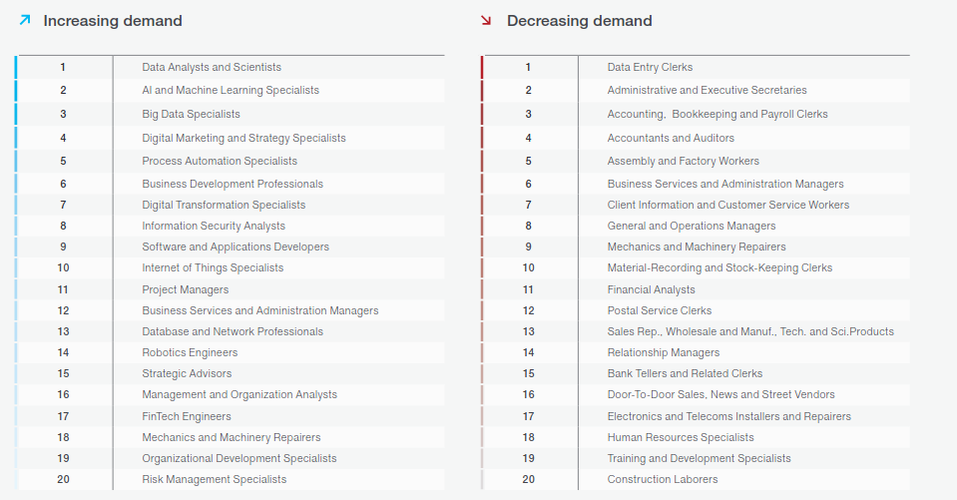
\includegraphics[width=1\textwidth]{images/Increasing_Jobs.png} 	%Incluyendo imagen Flow Core.
  \caption{Top 20 demanda de roles laborales en aumento y disminución para el año 2020, por participación de las empresas encuestadas por el \textit{Foro Económico Mundial}\cite{jobs_future}.}  
  \label{fig:Increasing_Jobs}
\end{figure}

\begin{figure}[H]    %[H] es para que se ubique justo debajo del texto anterior. 
  \centering
  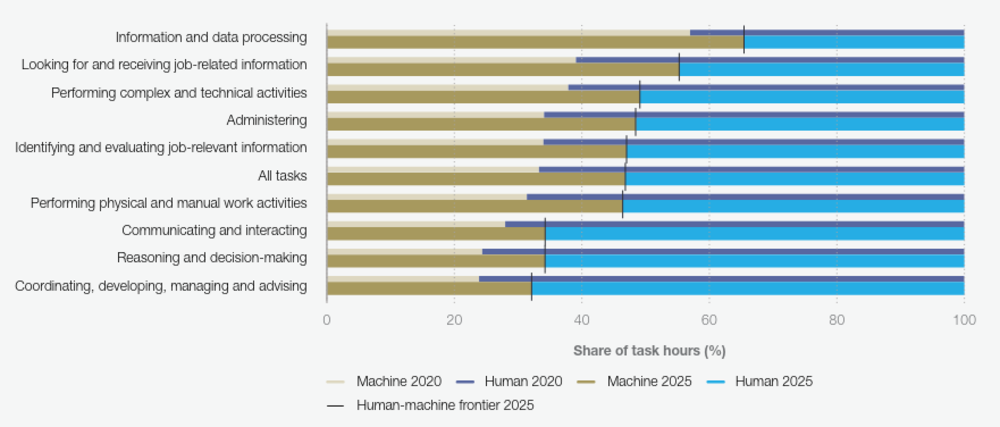
\includegraphics[width=1\textwidth]{images/Automatizacion.png} 	%Incluyendo imagen Flow Core.
  \caption{Porcentaje de tareas realizadas por humanos frente a máquinas, 2020 y 2025 (previsto),
por participación de las empresas encuestadas por el \textit{Foro Económico Mundial}\cite{jobs_future}.}  
  \label{fig:Automatizacion}
\end{figure}

El tema de este Proyecto de Tesis será desarrollar un \textit{sistema de lectura automática de Curriculum Vitae} accesible vía Web. La finalidad del mismo es ayudar al reclutador laboral a elegir a los mejores candidatos para los puestos laborales de IT que tenga disponible. Esta elección se realiza mediante el uso de algoritmos de machine learning y basándose, principalmente, en una medición de similitud entre textos: Curriculum Vitae de los candidatos por un lado, y descripciones de los puestos laborales de IT por el otro.

La medición de similitudes entre documentos de texto es uno de los problemas más cruciales del \textit{Procesamiento del Lenguaje Natural (NLP)} y es muy utilizado para el análisis de datos. Encontrar similitudes entre documentos se utiliza en varios dominios de NLP, tales como en sistemas de recomendación, de information retrieval (IR), de análisis de sentimientos, etc.\cite{Similarity_calculation}

Para que las máquinas puedan describir esta similitud entre documentos, se necesita definir una forma de medir matemáticamente la similitud, la cual debe ser comparable para que la máquina pueda identificar qué documentos son más (o menos) similares. Previamente a esto necesitamos representar el texto de los documentos en una forma cuantificable (que suele ser en forma vectorial), de modo que podamos realizar los posteriores cálculos de similitud sobre él. Una distancia pequeña entre los vectores significa un alto nivel de similitud, mientras que grandes distancias significan un bajo nivel de similitud\cite{Similarity_calculation}.

Por lo tanto, resumidamente los pasos necesarios para poder medir similitudes entre documentos son\cite{Similarity_calculation}:
\begin{enumerate}
\item Convertir cada uno de los documentos en un objeto matemático (vector).
\item Definir y emplear una métrica de distancia que será utilizada como nuestra medida de similitud entre los textos.
\end{enumerate}

\cleardoublepage    %Nueva página

En el sistema desarrollado, una vez obtenidas estas mediciones de similitud entre los Curriculum Vitae de los candidatos y las descripciones de los puestos laborales de IT mediante distintos algoritmos y técnicas de machine learning, estos valores se utilizarán para alimentar y generar \textit{un modelo de clasificación}, el cual nos servirá para lograr, en base a los valores de similitud de nuevos candidatos, clasificar qué tan similares son dichos candidatos con respecto a la descripción de un puesto de IT: similitud escasa, similitud media, similitud alta, similitud muy alta.\\

\subsection{Algoritmos y técnicas utilizadas.}

A continuación nombraremos resumidamente los algoritmos y técnicas de machine learning utilizadas para el desarrollo del \textit{sistema de lectura automática de Curriculum Vitae}. 

Como se mencionó en \textit{\nameref{Intro}}, el primer paso para lograr nuestra medición de similitudes entre documentos consiste en convertir los documentos en vectores: para esto se utilizaron los algoritmos de vectorización \textbf{TF-IDF} y \textbf{Word Embeddings}.

Para el segundo paso, definir y emplear métricas de distancia, se emplearon las técnicas \textbf{Cosine Similarity} y \textbf{Word Mover’s Distance (WMD)}.

Existen numerosas técnicas para medir distancias, las cuales serán detalladas en \textit{\nameref{Tecnicas_Simil_textos}}. Para este sistema se decidió utilizar una combinación entre Cosine similarity y WMD debido a:

\begin{itemize}
\item En el caso de Cosine similarity, se utilizó dicha técnica debido a que es una de las más tradicionales y ampliamente utilizadas para medir similitudes entre textos en varias aplicaciones\cite{similarity_survey, cosine_sim_1, cosine_sim_2, cosine_sim_3}.
\item En cambio, WMD es una técnica más nueva (2015)\cite{wmd_paper} que al momento de la encuesta realizada el 31 de Agosto del 2020\cite{similarity_survey} es la principal técnica utilizada para la medición semántica de la distancia entre textos.
\end{itemize} 
        
Como tercer y último paso, una vez obtenidas estas mediciones de similitud entre los Curriculum Vitae de los candidatos y las descripciones de los puestos laborales de IT, estos valores se utilizaron para alimentar un \textbf{algoritmo de clustering K-means} que a su vez, con sus datos de salida (4 clusters), alimentan a un \textbf{modelo de clasificación K-Nearest Neighbor (KNN)}.

Finalmente, con este modelo KNN logramos, en base a los valores de similitud de nuevos candidatos, clasificar qué tan similares son dichos candidatos con respecto a la descripción de un puesto de IT.

Estos algoritmos, técnicas y modelos utilizados serán detallados en las secciones posteriores, tanto teóricamente como en su implementación. 

\cleardoublepage    %Nueva página

\subsection{Objetivos del Proyecto.}

\subsubsection{Objetivo general.}

El objetivo de este Proyecto de Tesis es lograr un desarrollo, tanto teórico como práctico, de un \textit{sistema de lectura automática de Curriculum Vitae} accesible vía Web. La finalidad del mismo es ayudar al reclutador laboral a elegir a los mejores candidatos para los puestos laborales de IT que tenga disponible. Esta elección se realiza mediante el uso de algoritmos de machine learning y basándose, principalmente, en una medición de similitud entre textos:  
\begin{itemize}
\item los Curriculum Vitae de los candidatos por un lado, 
\item descripciones de los puestos laborales de IT por el otro.
\end{itemize} 

\subsubsection{Objetivos específicos.}
Los objetivos específicos de este Proyecto de Tesis son:
\begin{itemize}
\item Describir el estado del arte actual de los Sistemas de lectura y análisis de Curriculum Vitae en las fases de reclutamiento y selección laboral. 
\item Implementar un Sistema de lectura automática de Curriculum Vitae basado en la comparación y medición de similitudes entre textos, para finalmente obtener una visualización de los mejores candidatos para un puesto laboral de IT determinado.  
\item Aprender los conceptos y técnicas principales utilizadas dentro del procesamiento de lenguaje natural (NLP) aplicando técnicas de preprocesamiento y limpieza de textos.
\item Implementar diferentes técnicas para medir similitudes entre los textos (Cosine Similarity y  Word Mover's Distance -WMD-) y diferentes algoritmos de vectorización (TF-IDF y Word Embeddings), analizando su funcionamiento tanto teórica como matemáticamente, ventajas y desventajas.
\item Conocer, implementar e integrar el algoritmo de clustering K-means junto al algoritmo de clasificación KNN para obtener un modelo de clasificación de candidatos en base a las medidas de similitud entre los textos.
\item Evaluar los Frameworks disponibles para tener una UI \footnote{La interfaz de usuario o user inteface (UI) de una página web refiere a todo aquello tangible con lo que los usuarios interactúan de forma directa en la misma.} accesible vía web e integrar el mismo al Sistema.
\item Almacenar datos de candidatos, reclutadores y puestos laborales en una base de datos.
\end{itemize} 

\cleardoublepage    %Nueva página

\subsection{Alcance del Proyecto.}
El alcance de esta Tesis de Grado de Ingeniería incluye el desarrollo de conceptos de análisis de datos y machine learning, procesamiento de lenguaje natural, técnicas de preprocesamiento y limpieza de los datos, algoritmos de vectorización y técnicas para medir la similitud entre textos, algoritmos de clasificación y clustering, integración con frameworks, visualización de datos, y gestión de Base de Datos, de acuerdo a lo enunciado en los objetivos específicos.

\subsection{Organización.}
Este Proyecto de Tesis fue organizado para trabajarlo en tres secciones:

\begin{enumerate}
\item Análisis e investigación inicial. 

Esta sección abarca principalmente la parte teórica del trabajo, haciendo hincapié en el análisis e investigación de:
\begin{itemize}
	\item El estado del arte (actual y pasado) de los sistemas de lectura y análisis de Curriculum Vitae.
	\item Técnicas usadas para el procesamiento del lenguaje natural (NLP).
	\item Técnicas para medir similitudes entre textos: Cosine Similarity y WMD.
	\item Algoritmos de vectorización: TF-IDF y Word Embeddings.
	\item Algoritmos de machine mearning para tareas de clasificación (KNN) y clustering (K-means).
\end{itemize} 

Esta primera sección abarca los capítulos \textit{\nameref{2.ReclutamientolaboralenIT}}, \textit{\nameref{3.AlgoritmosdeMachineLearning}} y \textit{\nameref{4.NaturalLanguageProcessing}} de este Informe de Tesis. \\

\item Implementación de distintas técnicas y algoritmos para la obtención del modelo de clasificación KNN. 

Esta sección hace referencia a la aplicación práctica dentro del marco teórico desarrollado en la primera sección, mediante la realización de una serie de análisis en documentos de Jupyter Notebook \footnote{Aplicación cliente-servidor que permite crear documentos web en formato JSON que siguen un esquema versionado y una lista ordenada de celdas de entrada y de salida. Estas celdas albergan, entre otras cosas, código, texto (en formato Markdown), fórmulas y ecuaciones matemáticas. Estos documentos que se generan funcionan en cualquier navegador estándar.} utilizando Python \footnote{Lenguaje de programación interpretado y multiplataforma de código abierto, popularizado en los últimos años por su facilidad para trabajar con inteligencia artificial, big data, machine learning y data science, entre muchos otros campos en auge.}, para la obtención final de nuestro modelo de clasificación KNN capaz de clasificar, en base a los valores de similitud de nuevos candidatos, qué tan similares son dichos candidatos con respecto a la descripción de un puesto de IT: similitud escasa, similitud media, similitud alta, similitud muy alta. 

\cleardoublepage    %Nueva página

Los items que abarca esta sección son:

\begin{itemize}
	\item Obtención de sets de datos: curriculums vitae y descripciones laborales. 
	\item Preprocesamiento de los textos.
	\item Comparación entre textos y obtención de similitudes entre los mismos mediante el uso de las técnicas para medir distancias y obtener dichas similitudes (WMD y Cosine Similarity) y los algoritmos de vectorización (TF-IDF y Word Embeddings).
	\item Obtención del modelo de clasificación KNN utilizando como datos de entrada los clusters devueltos por el algoritmo K-means obtenidos en base a las mediciones de similitud previamente realizadas.
	\item Análisis y primeras visualizaciones de los resultados.
\end{itemize} 
 
Esta sección abarca el capítulo \textit{\nameref{5.Implementacion}} (desde \textit{\nameref{5.1.Obtenciondelmodelopredictivo}} hasta \textit{\nameref{5.4.Predicciondenuevasmuestrasyresultadosobtenidos}}) de este Informe de Tesis. \\

\item Integración al sistema web.

Esta última sección hace referencia a la reutilización de las funciones que contienen la lógica de los distintos algoritmos utilizados junto con el modelo de clasificación KNN obtenidos previamente en la sección 2, para integrar todo este conjunto en el sistema web que, a su vez, esta integrado a una base de datos relacional. De esta manera, el sistema cuenta con una interfaz gráfica permitiendo interactuar entre candidatos y reclutadores y, principalmente, permitiendo que el reclutador sea capaz de obtener un listado con los N candidatos más similes a un puesto determinado, y ordenados de mayor a menor de acuerdo a esta \textit{similitud}. Dicha \textit{similitud} representa el resultado obtenido de la clasificación por nuestro modelo KNN. 

Los items principales de esta sección son:
\begin{itemize}
	\item Definición de los usuarios que accederán al sistema.
	\item Definición de los datos que se almacenarán.
	\item Integración de frameworks y bases de datos.  
	\item Modelado, filtrado y visualización de los datos.
	\item Reutilización e integración al sistema de los algoritmos y del modelo KNN utilizados en la fase previa.	
	\item Evaluación del funcionamiento de todo el Sistema integrado.
\end{itemize} 

Esta última sección abarca el capítulo \textit{\nameref{5.Implementacion}} (desde \textit{\nameref{5.5.IntegracionalSistemaWeb}} hasta el final del capítulo) de este Informe de Tesis.
\end{enumerate}

\cleardoublepage    %Nueva página

\section{Reclutamiento y selección laboral.}\label{2.ReclutamientolaboralenIT}

En este capítulo se va a realizar una introducción a los procesos de reclutamiento y selección laboral, sus diferencias y diferentes tareas involucradas. Por último, se llevará a cabo un análisis del Estado de Arte actual de los sistemas de cribado (o más conocidos como sistemas de \textit{screening}) y se detallará el enfoque utilizado para este Proyecto.

\subsection{Introducción.}

Los procesos de \textit{reclutamiento y selección laboral} se han vuelto cruciales para el manejo de recursos humanos en el mundo moderno. Con las transformaciones digitales de las empresas y del mercado laboral en general, identificar los perfiles más acordes a las necesidades de la empresa se convirtió en uno de los retos más ambiciosos de Recursos Humanos, en especial cuando hablamos del \textit{Sector IT}, donde año tras año se van generando nuevos puestos de trabajo y estos mismos van creciendo en demanda. 

Los \textit{reclutadores}, dentro de un departamento de recursos humanos, son los encargados de llevar a cabo los procesos de \textit{reclutamiento} y \textit{selección} laboral. Uno de sus objetivos principales es buscar talento humano para cubrir los puestos de trabajo vacantes que tenga la empresa.

\subsection{Reclutamiento vs selección.}\label{SeleccionYReclutamiento}

El \textbf{reclutamiento} es el proceso de atracción, búsqueda, recolección e identificación de candidatos que encajan con la oferta de trabajo y, en definitiva, con la empresa. Como mencionan Anwar y Abdullah, \textit{``el reclutamiento es el proceso de descubrir y capturar candidatos calificados o apropiados para ocupar el puesto vacante''}\cite{seleccion_reclutamiento_2}.

El objetivo del reclutamiento es \textit{atraer}, \textit{buscar} e \textit{identificar} a los candidatos más adecuados y mejor calificados para el puesto disponible, según las necesidades de la empresa. 

El proceso de reclutamiento incluye las siguientes actividades\cite{seleccion_reclutamiento_2}:
\begin{itemize}
\item Identificación de las necesidades del puesto a cubrir. 
\item Análisis de la descripción y especificaciones del puesto.
\item Identificación de posibles fuentes de candidatos cualificados para el puesto.
\item Publicacion del puesto vacante en dichas fuentes.
\item Atracción de candidatos para aplicar al puesto.
\item Manejo apropiado en las respuestas y en los escrutinios a las postulaciones.
\end{itemize}

\cleardoublepage    %Nueva página

En cambio, la \textbf{selección} es un proceso posterior al reclutamiento, donde se evalua más detalladamente y se entrevista a los candidatos para el trabajo en particular. Como mencionan Rahman y Abdullah, \textit{``la selección es un proceso de evaluar y entrevistar a los candidatos para un trabajo en particular y seleccionar a la persona adecuada para el puesto correcto''}\cite{seleccion_reclutamiento_2}.

El objetivo de la selección es \textit{elegir} y \textit{hacer efectiva la contratación} del candidato más adecuado y mejor calificado para el puesto disponible, según las necesidades de la empresa. Este procedimiento particiona a los candidatos en dos secciones: a los que se les ofrecerán el trabajo, y a los que se descartarán.

El proceso de selección incluye las siguientes actividades\cite{seleccion_reclutamiento_2}: 
\begin{itemize}
\item Recepción de la aplicación al puesto.
\item Cribado o Screening de los candidatos, lo que permite avanzar con los candidatos adecuados y descartar a los no adecuados para el puesto.
\item Entrevistas a los candidatos.
\item Manejo de tests a los candidatos, tales como tests médicos o psicológicos. 
\item Manejo de exámenes a los candidatos, tales como exámenes técnicos, de aptitud, inteligencia, performance, etc.
\item Evaluación de las referencias de los candidatos.
\item Decisión final acerca de la contratación o no contratación del candidato.
\end{itemize}

Como conclusión, podemos decir que en la fase de \textbf{reclutamiento} se trata de encontrar muchos candidatos que cumplan con los requisitos de la oferta; mientras que en la etapa de \textbf{selección} se debe elegir al mejor candidato para las necesidades de la empresa. 

\cleardoublepage    %Nueva página

\subsection{Evolución de los procesos de reclutamiento y selección laboral.}
Los procesos de reclutamiento y selección laboral fueron evolucionando a lo largo del tiempo\cite{trabajos_relacionados_10}:

En los modelos de reclutamiento y selección de \textbf{primera generación}, las empresas anunciaban sus vacantes de puestos laborales en diarios, revistas, radio y en televisión. Los candidatos enviaban sus currículums por correo postal y los mismos se clasificaban manualmente: algo muy tedioso y que llevaba mucho tiempo en realizar. Una vez \\ preseleccionados los candidatos, los reclutadores llamaban a los mismos para realizar las rondas de entrevistas. 

Luego pasamos a la \textbf{segunda generación}. En esta época las empresas comenzaron a crecer y también lo hicieron las necesidades de reclutamiento y selección. Las empresas empezaron a subcontratar sus procesos de reclutamiento y selección, naciendo de esta manera las consultoras o agencias de contratación. Estas consultoras requerían que los candidatos cargaran sus currículums en sus sitios web en formatos particulares. Luego, las consultoras revisaban los datos de los candidatos y preseleccionaban a los mismos para la empresa. El gran inconveniente de este proceso fue que habían numerosas consultoras y cada una tenía su propia y única forma de selección, no era un proceso uniforme.

Para intentar superar los problemas anteriores, se llegó a una \textbf{tercera generación}, en la que estamos actualmente. En esta generación se crearon, y siguen creándose, una gran cantidad de herramientas de Software que utilizan algoritmos inteligentes y permiten automatizar y gestionar información de los candidatos de una manera mucho más intuitiva. Estos sistemas ayudan a los reclutadores dentro de las empresas y consultoras a analizar la información de cualquier Curriculum Vitae y clasificarlos o listarlos en función de los puestos disponibles. De esta manera, cuando el reclutador publica una oferta de trabajo, estos sistemas clasifican o listan a los currículums basándose en distintas métricas (por ejemplo palabras clave) mostrando así los candidatos más relevantes para la empresa o consultora.

\cleardoublepage    %Nueva página

\subsection{Cribado o screening.}  

Como vimos anteriormente en \textit{\nameref{SeleccionYReclutamiento}}, el screening (o tambien conocido como cribado) es una etapa del proceso de selección. 
En esta etapa los reclutadores revisan los Currículums Vitae que fueron recibiendo por parte de los candidatos, y \\ preseleccionan a los que mejor se adapten a los requisitos de la oferta de empleo de la empresa. Este proceso es muy importante dentro del proceso de selección, ya que permite valorar en ese momento si el candidato es apto para continuar en el proceso de selección o, en caso contrario, si el mismo se descarta por no considerarlo adecuado para el puesto.

\subsubsection{Screening manual vs screening automatizado}  

Si el proceso de screening sigue el modelo tradicional y se realiza manualmente, es un proceso muy tedioso y que lleva mucho tiempo por parte del reclutador, el cual tiene que evaluar una gran cantidad de Curriculums Vitae. Existe un estudio\cite{estudio_eye_tracking} relizado en 2018 por Ladders Inc., empresa lider en sitios de carrera, donde se estudió cuánto tiempo en promedio tarda un reclutador en dar una primera vista rápida a un Curriculum Vitae de un candidato. Se descubrió que este tiempo es, en promedio, de 7.4 segundos. Este es el tiempo en el que el reclutador decide inicialmente si el candidato sigue (o no) con el proceso de selección.

Sin embargo, este tiempo es engañoso: ya que este estudio fue realizado con la aplicación de muchos Curriculums vitae que no cumplian con los criterios mínimos para calificar a los puestos; es por esto que los reclutadores realizaban una primer vista rápida y los descartaban (o no) a los pocos segundos. Si las aplicaciones provenieran de Curriculums Vitae que cumplan con los requisitos mínimos del puesto, este tiempo de observación sería mucho mayor, ya que el reclutador examinaría con mayor detalle los curriculums.

Adicionalmente, este estudio tampoco tiene en cuenta el tiempo consumido por el reclutador al comparar el Curriculum Vitae del candidato con la descripción o requisitos del puesto laboral, por lo que el tiempo en realizar un screening manual se incrementaría significativamente.

Otra de las desventajas al considerar el screening como un proceso manual, es que muchos son los factores que pueden influir al reclutador en el momento de tomar la decisión de descarte o selección del candidato, ya sea cansancio por el volumen de los curriculums ya revisados, la estructura, elementos discriminatorios o información incompleta dentro de los mismos, etc. Es por esto que las probabilidades de descartar prematuramente a un candidato válido son muy altas.

Frente a estas desventajas del modelo tradicional y poco eficiente del screening manual existe una solución: la \textit{automatización}. Actualmente existen sistemas automatizados y basados en Inteligencia Artificial que permiten realizar el screening de un volumen importante de curriculums en unos pocos segundos (Ver \textit{\nameref{Estado_del_arte}}). De esta manera, el proceso de screening no estaría afectado a factores externos que puedan influir en la decisión del reclutador, y además la herramienta sería capaz de entregar un listado justificado de los mejores candidatos para la siguiente fase del proceso en un tiempo relativamente corto.

\cleardoublepage    %Nueva página

Uno de los beneficios potenciales de utilizar sistemas automatizados e inteligentes en los procesos de screening es el acortamiento de los ciclos de contratación, lo que hace que la organización responda mejor a los solicitantes y sea más capaz de competir con otras organizaciones por los mejores candidatos\cite{seleccion_reclutamiento_1}.  

Muchos gerentes de recursos humanos depositan sus esperanzas en la tecnología y las herramientas automatizadas e inteligentes: desde el aumento de la eficiencia y la reducción de costos hasta el aumento de las aplicaciones de candidatos y la estandarización de todos sus sistemas de selección\cite{seleccion_reclutamiento_1}.

\subsection{Sistemas de screening: Estado del arte.}\label{Estado_del_arte}

Tal como mencionamos en la sección anterior, un sistema de screening automatizado e inteligente nos permite entregar al reclutador una shortlist con los candidatos que mejor se adaptan a los requisitos de la oferta de empleo de la empresa. De esta manera, al realizar dicha preselección de candidatos, el reclutador podrá seguir con las etapas posteriores de selección o podrá realizar otro screening manual para descartar a otros candidatos.

A continuación detallaremos una serie de trabajos de relevancia (tanto de implementación como de investigación) donde se utilizaron distintos enfoques para desarrollar o sugerir un desarrollo de un sistema de screening de candidatos.

En \cite{trabajos_relacionados_1} utilizaron el \textit{algoritmo KNN} para clasificar los curriculums de los candidatos en diferentes categorías, y luego utilizaron la métrica de similitud \textit{Cosine Similarity} para averiguar qué tan cerca está el curriculum del candidato con respecto a la descripción de los puestos, y realizar un ranking acorde a estos resultados.

En \cite{trabajos_relacionados_2} utilizaron una herramienta inteligente llamada \textit{EXPERT mapping-based candidate screening} que utiliza  \textit{ontology mapping}\footnote{La \textit{ontología (ontology)} permite la especificación explícita de un dominio de discurso, que permite acceder y razonar sobre el conocimiento de un agente. Las ontologías elevan el nivel de especificación del conocimiento, incorporando semántica a los datos.
El \textit{mapeo de ontologías (ontology mapping)} es el proceso mediante el cual dos ontologías se relacionan semánticamente a nivel conceptual y las instancias de ontología de origen se transforman en entidades de ontología de destino de acuerdo con esas relaciones semánticas.\cite{ontology_mapping} } para crear un sistema automatizado para el screening inteligente de candidatos. 

En \cite{trabajos_relacionados_3} y \cite{trabajos_relacionados_4} también se utilizan sistemas basados en \textit{ontologías} para extraer datos de curriculums y realizar macheos con los puestos disponibles.

En \cite{trabajos_relacionados_5} sugieren un método de matching basado en un \textit{modelo probabilístico} para ser utilizado en la selección y recomendación de candidatos. 

En \cite{trabajos_relacionados_6} se propuso un aistema automatizado de screening de currículums que usa \textit{Vector Space Model}\footnote{Modelo algebraico para representar documentos de textos en lenguaje natural de una manera formal mediante el uso de vectores de identificadores. Es utilizado para la recuperación, filtrado, indexado y cálculo de relevancia de información.} para machear cada curriculum con la descripción del puesto correspondiente y \textit{cosine similarity} como medida de similitud.

\cleardoublepage    %Nueva página

En \cite{trabajos_relacionados_7} y \cite{trabajos_relacionados_8} se propuso un sistema para el screening de candidatos, para el cual se utiliza \textit{cosine similarity}, \textit{KNN} y un \textit{sistema de recomendación basado en contenido (Content Based Filtering, CBF)} para buscar los curriculums más cercanos a la descripción del puesto.

En \cite{trabajos_relacionados_9} se propuso un sistema para el ordenamiento y clasificación de currículums utilizando el concepto de inteligencia artificial (sin especificar qué algoritmos o técnicas específicas se deberían usar). Lo que se propuso fue un esquema de trabajo para luego seguir con la implementación del sistema; el cual permitiría clasificar a todos los currículums de acuerdo con los requisitos de la empresa y los enviaría a Recursos Humanos para su posterior consideración.

En \cite{trabajos_relacionados_10} se diseñó un sistema que ayuda a los reclutadores a seleccionar los curriculums basados en la descripción del trabajo. Ayuda en un proceso de contratación fácil y eficiente al extraer los requisitos automáticamente. Este sistema utiliza un \textit{modelo NER (Named entity recognition)} \footnote{Subtarea de \textit{information extraction (IE)} que permite buscar y categorizar entidades específicas en un cuerpo o cuerpos de textos.}.

En \cite{trabajos_relacionados_11} y \cite{trabajos_relacionados_12} se implementan sistemas basados en \textit{semantic anotation}\footnote{Proceso de etiquetado de documentos con conceptos relevantes. Los documentos se enriquecen con metadatos que permiten vincular el contenido a los conceptos, descritos en un gráfico de conocimiento. Esto hace que el contenido no estructurado sea más fácil de encontrar, interpretar y reutilizar.} y \textit{ontologías}, permitiendo realizar macheos entre las ofertas de trabajo y los curriculums de los candidatos.

En \cite{trabajos_relacionados_13} se utiliza \textit{relevance feedback}\footnote{Característica de algunos sistemas de \textit{information retrieval (IR)}. La idea de relevance feedback es tomar los resultados que se devuelven inicialmente de una consulta/query determinada, recopilar los comentarios de los usuarios y usar información para evaluar si esos resultados son relevantes o no para realizar una nueva consulta/query.} para la implementación de un sistemas que intenta encontrar a los mejores candidatos para las distintas ofertas de trabajo.

\textit{Paul Resnick} y \textit{Hal R. Varian} fueron pioneros en los \textit{sistemas de recomendación}\footnote{Un \textit{sistema de recomendación} es una subclase de los sistemas de \textit{Information filtering (IF)} que busca predecir la calificación o la preferencia que un usuario le puede dar a un artículo. En palabras simples, es un algoritmo que sugiere artículos relevantes para los usuarios.}\cite{sistema_recomendacion}.
En \cite{trabajos_relacionados_14} y \cite{trabajos_relacionados_15} se utilizaron dichos \textit{sistemas de recomendación} junto a otros algoritmos para implementar aplicaciones de screening y clasificación de candidatos. Esto es debido a que, dado que el perfil del candidato es necesario para un puesto en particular, la forma en que se comparan los curriculums de los candidatos es muy similar a un sistema de recomendación. 

\cleardoublepage    %Nueva página

\subsection{Enfoque del Proyecto.}

Como vimos en la sección anterior, hay cientos de enfoques y combinaciones posibles para realizar un sistema de screening automático e inteligente.

El enfoque elegido para este Proyecto de Tesis fue realizar un sistema híbrido que utilice técnicas de mediciones de similitud entre los curriculums de los candidatos y las descripciones de los puestos disponibles, junto con técnicas de machine learning (de clustering y clasificación). 

Como métricas de medición de similitud se utilizó una de las más comúnmente usadas, \textit{similitud del coseno}, y una métrica que \textbf{no se usó en ninguno de los trabajos anteriores} pero, que sin embargo, es muy reciente y prometedora, y es la principal técnica utilizada para la medición semántica de la distancia entre textos, \textit{Word Mover's Distance (WMD)}. Estas métricas serán explicadas más en detalle en las secciones posteriores (Ver \textit{\nameref{Tecnicas_Simil_textos}}).

Una vez utilizadas estas mediciones de similitud se utilizaron algoritmos de machine learning: un algoritmo de clustering K-means, y luego un modelo de clasificación KNN. 

Además del uso de \textit{Word Mover's Distance}, otro aspecto distintivo de este sistema es que se realizó una \textbf{integración a una interfaz web}, la cual la mayoría de los sistemas descriptos anteriormente no poseen. De esta manera, mediante la interfaz web se logra una interacción entre usuarios candidatos y reclutadores y, principalmente, permite que el reclutador sea capaz de visualizar un listado con los N candidatos más similes a un puesto determinado.

Por último, cabe destacar que los trabajos anteriormente mencionados no tienen un fácil acceso a los datasets ni al código que utilizaron para dichos sistemas, por lo que seguir el trabajo de ellos aplicando las mejoras que mencionan en sus artículos es una tarea casi imposible. En cambio, \textbf{este sistema será de código abierto}: los datasets, modelos y códigos utilizados estarán disponibles en Github y Git LFS\footnote{\url{https://github.com/FedericoCalonge/automatic_reading_of_CVs_using_text_similarity}}.

\cleardoublepage    %Nueva página\\

\section{Algoritmos de Machine Learning.}\label{3.AlgoritmosdeMachineLearning}

\subsection{Introducción.}
Continuando con el marco teórico de esta Tesis, es necesario explicar qué es \textit{machine learning (ML)} y cómo se pueden clasificar a los distintos algoritmos y modelos según su tipo de aprendizaje, haciendo énfasis en los algoritmos K-Nearest Neighbor (KNN) y K-means, y el modelo de Redes Neuronales. Estas técnicas son las que se utilizarán en la implementación del proyecto.

Además, detallaremos la importancia de la separación de los datos y mencionaremos cuáles son los pasos a seguir para implementar un modelo de ML teniendo en cuenta algunos de los problemas clásicos que pueden afectar a nuestros resultados.

\subsection{Machine Learning (ML).} 

La \textbf{Inteligencia Artificial (IA)} es una disciplina dentro de las ciencias de la computación que consiste en el desarrollo de algoritmos\footnote{Un algoritmo informático es un conjunto de instrucciones definidas, ordenadas y acotadas para resolver un problema, realizar un cálculo o desarrollar una tarea.} que imiten el razonamiento humano, teniendo la capacidad de solucionar problemas que comúnmente resuelve la inteligencia natural pero de la manera más eficiente posible. 
Esencialmente, la IA permite que las máquinas puedan actuar e implementar distintas tareas que están fuera del alcance de los humanos \cite{intro_algos_ML}.

\textbf{Machine Learning (ML)} o \textbf{Aprendizaje Automático} es un subconjunto de la Inteligencia Artificial que se encarga de construir algoritmos que aprenden a hacer algo útil a partir de los datos. 
Como ML es un subconjunto de IA, esto implica que todos los algoritmos de ML son técnicas de inteligencia artificial, pero no todos los métodos de inteligencia artificial califican como algoritmos de ML.

El objetivo principal de ML es permitir que las computadoras aprendan sin intervención o asistencia humana.
Esencialmente, los algoritmos de ML aprenden \textit{patrones} ocultos basados en datos históricos de entrada, los cuales posteriormente utilizan para aprender a clasificar la información o realizar predicciones relacionadas con el problema que se quiera resolver. 

Los algoritmos de ML hoy en día se usan en todo tipo de aplicaciones: en Amazon para recomendarnos qué productos comprar, en Twitter para recomendarnos qué usuarios seguir, en Google para predecir qué páginas son las más relevantes para una consulta, en Facebook para reconocer qué fotos contienen rostros de personas, en el mercado inmobiliario para predecir los precios de las propiedades, en el mercado de valores para predecir el precio de las acciones, etc. Son tantas las aplicaciones de ML en la industria que se ha producido una verdadera explosión del tema en los últimos años\cite{apunte_uba}.

\cleardoublepage
\subsubsection{Aprendizaje supervisado y no supervisado.}

Podemos dividir a ML en dos grandes categorías: aprendizaje supervisado y aprendizaje no supervisado. Resumidamente, la diferencia entre estas dos categorías es la existencia de etiquetas (labels) en el subconjunto de datos de entrenamiento (Ver \textit{\nameref{Separacion datos}}).

\begin{itemize}
\item En el \textbf{aprendizaje supervisado}, el modelo es entrenado utilizando datos que están “etiquetados”. Esto quiere decir que el set de datos que es utilizado para enseñar al algoritmo tiene una etiqueta (o label) que define la respuesta/salida correcta. 

Analizándolo matemáticamente, este proceso puede ser representado por una variable de entrada $x$ y una conocida variable de salida $y$, donde se usa un algoritmo $f$ para que aprenda a predecir resultados para aquellos nuevos datos que no tienen etiqueta.

$$y=f(x)$$

Los algoritmos de aprendizaje supervisado se utilizan para resolver problemas de \textbf{clasificación} y de \textbf{regresión}.

\item El \textbf{aprendizaje no supervisado}, en cambio, se refiere al proceso de entrenamiento de un modelo de machine learning sin un set de datos etiquetado. Este tipo de aprendizaje es una rama muy importante en Data Science ya que, al trabajar solo con datos sin necesidad de tener un ”label” para los mismos, únicamente necesitamos los datos en crudo y estos en general son mucho más fáciles de conseguir que datos ya previamente clasificados. Por ejemplo, las aplicaciones de redes sociales tienen grandes cantidades de datos sin etiquetar.  

El objetivo de este método es experimentar con el conjunto de datos (los cuales contienen muchas características) y luego aprender propiedades útiles de la estructura de dicho conjunto de datos. Matemáticamente se cuenta con un dataset de entrenamiento de variables de entrada $x$ pero no se conoce su salida. 

$$\mbox{¿}?=f(x)$$

Los algoritmos de aprendizaje no supervisado se utilizan para resolver problemas de \textbf{clustering}.
\end{itemize}

\cleardoublepage
En la Figura \ref{fig:Clasif_algoritmos} se detalla un resumen de la división en las categorías de ML y su sub-división en modelos de clasificación, regresión y agrupación (clustering). 

\begin{figure}[H]    %[H] es para que se ubique justo debajo del texto anterior. 
  \centering
  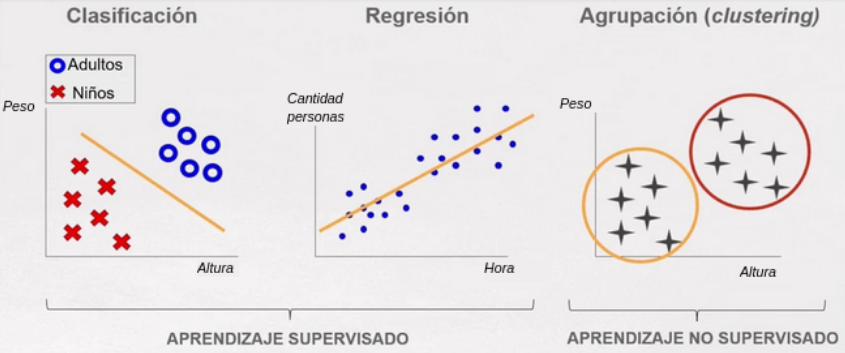
\includegraphics[width=1\textwidth]{images/Clasificacion_algoritmos.png}
  \caption[Tipos de aprendizaje en ML]{Tipos de aprendizaje en ML\protect\footnotemark}  
  \label{fig:Clasif_algoritmos}
\end{figure}

\footnotetext{Sitio Web. \textit{Modelos de Machine Learning}. \url{https://openwebinars.net/blog/modelos-de-machine-learning/}. (Consultado el 30 marzo de 2022).}

\paragraph{Regresión.}

En un problema de regresión se intenta predecir el valor de una variable numérica y continua a partir de un cierto conjunto de datos. 

En general contamos con un set de entrenamiento en el cual conocemos el valor de la variable que queremos predecir. El objetivo es entonces construir un modelo que nos permita predecir el valor de nuestra variable de salida a partir de datos nuevos. Dicho de otra forma, lo que se hace es buscar una función que represente los datos de entrenamiento y que permita generalizar correctamente\footnote{Generalizar es la capacidad de nuestro modelo de ML de obtener buenos resultados con datos nuevos reconociendo patrones generales de los datos de entrenamiento en lugar de reconocer particularidades específicas.}.

El caso más simple es la regresión lineal (observado previamente en la Figura \ref{fig:Clasif_algoritmos}), en el cual nuestro modelo es una recta, la recta que mejor se ajusta a los puntos de nuestro set de entrenamiento. En este ejemplo se intenta predecir la cantidad de personas en un lugar a una hora determinada. 

Los problemas de regresión pueden usarse para realizar distintas predicciones, ya sea el valor de las acciones en el mercado de valores, predecir el costo de una propiedad, estimar las ganancias de un negocio, etc. 

Las claves para identificar un problema de regresión\cite{apunte_uba} son las siguientes:
\begin{itemize}
\item Queremos predecir una variable que es numérica y continua.
\item Contamos con un set de entrenamiento para el cual conocemos el valor de dicha variable.
\end{itemize}

\cleardoublepage
\paragraph{Clasificación.}\label{clasificacion}

En los problemas de clasificación la variable que se intenta predecir no es continua sino discreta, frecuentemente tiene pocos valores posibles y en muchos casos los valores posibles son solo dos: clasificación binaria\footnote{Un caso típico de la clasificación binaria es un problema de análisis de sentimiento, donde queremos saber si un cierto texto es positivo o negativo, es decir si habla bien o mal de un cierto tema. Como set de entrenamiento entonces deberíamos contar con textos para los cuales ya conocemos su sentimiento.}. La idea general es la misma que antes, para este caso contamos con un set de entrenamiento en el cual para cada dato conocemos la clase a la cual pertenece el mismo, y queremos construir un modelo que nos permita clasificar automáticamente datos nuevos cuya clase desconocemos.

Por ejemplo, en la Figura \ref{fig:Clasif_algoritmos}, observamos que tenemos una serie de personas, de las cuales contamos con su peso y altura, y queremos clasificarlas en adultos o niños. Lo que va a hacer un modelo de clasificación es aprender dónde están estos puntos y crear un clasificador que, para nuevos datos de entrada, consiga segmentarlos correctamente en adultos o niños.

Otras aplicaciones, por ejemplo, podrían ser analizar si las reviews de un producto son buenas o malas, medir la actitud del público en general ante determinadas noticias por los comentarios que existen en redes sociales, clasificar si un email es spam o no lo es, etc. 

Las claves para reconocer un problema de clasificación\cite{apunte_uba} son:
\begin{itemize}
\item Queremos determinar la clase / grupo  a la que pertenece cada dato.
\item La clase es una variable discreta con un set de valores posibles limitado y definido.
\item Contamos con un set de entrenamiento para el cual conocemos los datos y a qué clase pertenecen.
\end{itemize}

\cleardoublepage
\paragraph{Agrupación (clustering).}\label{agrupacion}

En un problema de clustering contamos con datos que queremos dividir en grupos de forma automática. Estos datos no tienen etiquetas, no sabemos a qué grupo pertenecen. Lo que hace un algoritmo de clustering es intentar buscar agrupaciones en los datos, creando de esta forma clusters\footnote{Cluster, o grupo, es un conjunto de objetos que son ”similares” entre ellos y ”diferentes” de los objetos que pertenecen a los otros grupos. La palabra cluster viene del inglés y significa agrupación. Desde un punto de vista general, el cluster puede considerarse como la búsqueda automática de una estructura o de una clasificación en una colección de datos no etiquetados.} con características similares. En algunos casos la cantidad de clusters la debemos indicar previamente y en otros el algoritmo es capaz de determinarla por sí mismo.

En el ejemplo de la Figura \ref{fig:Clasif_algoritmos}, podemos ver que se agrupan los puntos de la misma forma que en el problema de clasificación. La diferencia es que en este caso no sabemos si se trata de adultos o niños, sino que es el propio algoritmo el que va a identificar que hay dos grupos, y nosotros somos los que tenemos que interpretar los resultados. 

Otros ejemplos de clustering podrían ser agrupar películas automáticamente de forma que queden juntas las que son de un mismo género; o la detección de comunidades en una red social, el cual es un típico problema de clustering en donde los puntos son los usuarios y queremos agruparlos automáticamente en comunidades. De esta forma podemos descubrir grupos de usuarios que tienen un cierto interés en común aun sin saber exactamente cuál es dicho interés.

Las claves para reconocer un problema de clustering\cite{apunte_uba} son:
\begin{itemize}
\item Contamos con un set de datos y queremos agruparlos en clusters/grupos.
\item No son necesarios labels.
\end{itemize}

\cleardoublepage

\paragraph{Algoritmos más conocidos.}

Resumidamente, en la Figura \ref{fig:Diagrama_algoritmos} se detallan los algoritmos más conocidos para las distintas clasificaciones de machine learning previamente explicadas. 

\begin{figure}[H]    %[H] es para que se ubique justo debajo del texto anterior. 
  \centering
  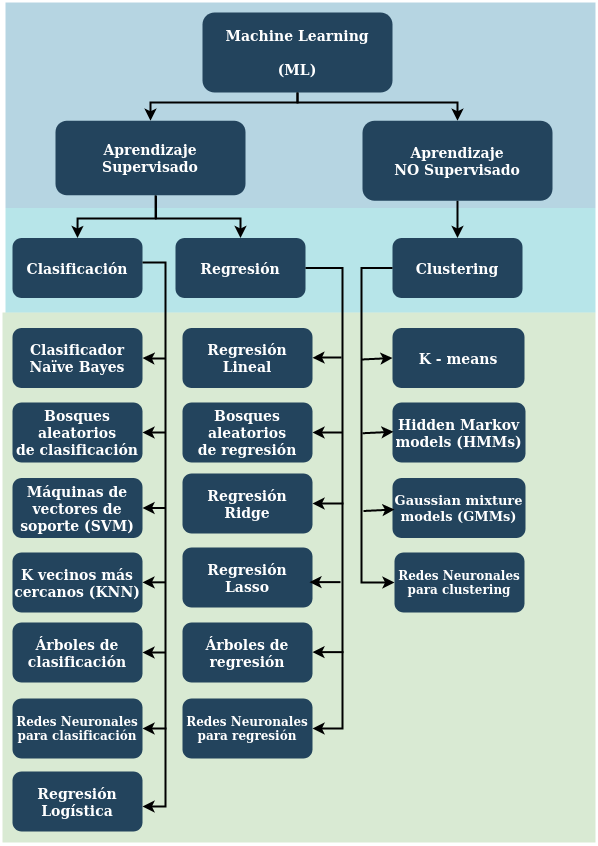
\includegraphics[width=0.8\textwidth]{images/Diagrama_algoritmos.png}
  \caption{Algoritmos de machine learning más conocidos}  
  \label{fig:Diagrama_algoritmos}
\end{figure}

Cabe destacar que algunos algoritmos se pueden adaptar para resolver problemas de otro tipo al cual están inicialmente categorizados. Por ejemplo, KNN que está categorizado como un algoritmo de clasificación, también se puede utilizar para resolver problemas de regresión. Otro caso conocido es Support Vector Regression (SVR), que utiliza las bases de Máquinas de vectores de soporte (SVM) para resolver problemas de regresión.

\cleardoublepage

\subsubsection{Aprendizaje transductivo}

Existe una cierta relación entre los problemas de clustering y de clasificación, por ejemplo dado un problema de clasificación podríamos aplicar clustering primero y luego clasificar a cada punto de acuerdo al cluster al cual pertenece en base a la clase mayoritaria de dicho cluster. Este procedimiento no es muy frecuente pero es conveniente tenerlo en cuenta porque permite entender el funcionamiento de ciertos algoritmos que combinan las propiedades de un problema de clustering y uno de clasificación.

Una aplicación que combina clustering (aprendizaje no supervisado) y clasificación (aprendizaje supervisado) es la que denominamos \textbf{Aprendizaje transductivo}\cite{aprendiz_transd}\cite{apunte_uba} . De esta manera, para predecir nuevos datos no etiquetados se utilizan los datos previamente etiquetados, así como los datos sin etiquetar, como forma de ayuda a un clasificador tradicional.

Consideremos el ejemplo de la Figura \ref{fig:Transductivo_1}. Aquí tenemos solo dos puntos clasificados, uno clasificado como ``blanco'' y el otro como ``negro''. Sin mayor información el punto marcado con el signo de pregunta, cuya clase desconocemos, quedaría clasificado como ``blanco'' ya que está mucho mas cerca del punto blanco que del punto negro.

\begin{figure}[H]    %[H] es para que se ubique justo debajo del texto anterior. 
  \centering
  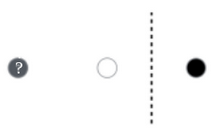
\includegraphics[width=0.5\textwidth]{images/Transductivo_1.png}
  \caption{Aprendizaje transductivo}  
  \label{fig:Transductivo_1}
\end{figure}

En la Figura \ref{fig:Transductivo_2} al agregar puntos cuya clase desconocemos, vemos que en nuestros datos existen dos clusters. De esta manera, si tenemos que asociar cada cluster con un color entonces el de arriba es ``negro'' y el de abajo es ``blanco'', ya que el punto negro pertenece al cluster de arriba y el blanco al de abajo. De este modo, el punto que inicialmente consideramos blanco, con esta nueva información de clusters, sería considerado negro.

\begin{figure}[H]    %[H] es para que se ubique justo debajo del texto anterior. 
  \centering
  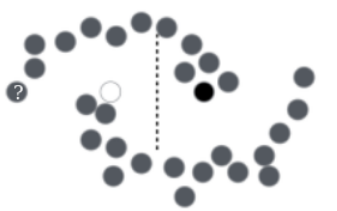
\includegraphics[width=0.5\textwidth]{images/Transductivo_2.png}
  \caption{Aprendizaje transductivo}  
  \label{fig:Transductivo_2}
\end{figure}

El aprendizaje transductivo es un área muy nueva dentro de Data Science y que sin dudas merece ser explorada.

En este proyecto de Tesis se utilizará el aprendizaje transductivo para lograr inicialmente una clusterización de nuestros candidatos en 5 grupos mediante un algoritmo de clustering (K-means), y luego se realizará una clasificación mediante un algoritmo de clasificación (KNN). 

\subsubsection{Separación de los datos.}\label{Separacion datos}

Dos conceptos importantes que mencionaremos a lo largo del informe son: los “datos de entrenamiento” y los “datos de prueba”.

Como mencionamos anteriormente, los algoritmos de machine learning aprenden de los datos con los que los entrenamos. A partir de ellos, intentan encontrar o inferir el patrón que les permita predecir el resultado para un nuevo caso. Pero, para poder calibrar si un modelo funciona, necesitaremos probarlo con un conjunto de datos diferente. Por ello, en todo proceso de aprendizaje automático, los datos de trabajo se deben dividir mínimamente en dos partes:

\begin{itemize}
\item Los \textbf{datos de entrenamiento} son los datos que usamos para entrenar un modelo. La calidad de nuestro modelo de aprendizaje automático va a ser directamente proporcional a la calidad de estos datos. Por ello son muy importantes las tareas de limpieza y preprocesamiento de los mismos.
\item Los \textbf{datos de prueba o evaluación} son los datos que nos “reservamos” para comprobar si el modelo que hemos generado a partir de los datos de entrenamiento “funciona”.  Es decir, si las respuestas predichas por el modelo para un caso totalmente nuevo son acertadas o no.
\end{itemize}


Es importante que el conjunto de datos de prueba tenga un volumen suficiente como para generar resultados estadísticamente significativos, y a la vez, que sea representativo del conjunto de datos global. Normalmente el conjunto de datos se suele dividir en un \textbf{70\%/80\% de datos de entrenamiento} y un \textbf{30\%/20\% de datos de prueba}, pero se puede variar la proporción según el caso\cite{apunte_uba}. 


\cleardoublepage
\subsubsection{¿Cómo implementar un modelo de ML?}

Resumidamente, los pasos a seguir para implementar un modelo de ML y utilizarlo para realizar predicciones sobre los datos son los siguientes:
\begin{itemize}
\item Paso 1: Recolección de Datos.
\item Paso 2: Preparación y preprocesamiento de los datos.
\item Paso 3: Elección del modelo de ML.
\item Paso 4: Entrenamiento del algoritmo.
\item Paso 5: Evaluación del modelo.
\item Paso 6: Parameter Tuning o configuración de parámetros.
\item Paso 7: Utilizando nuestro modelo.\\
\end{itemize}

A continuación detallaremos en mayor detalle los mencionados pasos.

\begin{itemize}
\item Paso 1: Recolección de Datos.

Dada la problemática que deseemos resolver mediante algoritmos de ML, nuestro primer paso será recolectar los datos que utilizaremos posteriormente para “alimentar” a dicho algoritmo. 

En este paso hay que tener muy en cuenta la calidad y cantidad de información que consigamos ya que impactará directamente en lo bien o mal que luego funcione nuestro modelo. Estos datos los podemos sacar de bases de datos, planillas de cálculo, utilizando técnicas de web scraping\footnote{Proceso dentro de Data Science que se utiliza para la extracción de datos de sitios web simulando cómo navegaría un ser humano por los mismos.} o mediante APIs\footnote{API o interfaz de programación de aplicaciones, es un conjunto de métodos o funciones que ofrece cierta biblioteca para ser utilizada por otro software como una capa de abstracción.} para recopilar información de manera automática de diversas fuentes de Internet, etc.\\

\item Paso 2: Preparación y preprocesamiento de los datos.

En este paso generalmente se realizan visualizaciones de los datos y se revisa si existen correlaciones entre las distintas “features”\footnote{Features generalmente son las columnas de nuestro dataframe, archivo o base de datos -dependiendo cómo almacenamos nuestros datos-.} de nuestros datos. Al pre-procesar nuestros datos nos referimos a normalizar los mismos: eliminando duplicados y realizando distintas correcciones de errores. El preprocesamiento de datos usualmente tiene un impacto significativo en la performance de generalización de nuestro algoritmo de machine learning\cite{preprocessing}. 

\cleardoublepage
En esta etapa, además, es importante \textbf{separar} nuestros datos en dos grupos:
\begin{itemize}
\item un set de entrenamiento.
\item un set de prueba. 
\end{itemize}

Como mencionamos previamente, el set de test en general es un 20\% o 30\% del set de entrenamiento. Esta partición de los datos en estos dos conjuntos diferenciados permite generar el modelo a partir de los datos de entrenamiento para después comprobar su eficiencia con los datos reservados para test.\\

\item Paso 3: Elección del modelo de ML.

Una vez obtenidos y preprocesados estos datos, lo que se hace es \textbf{elegir el modelo de ML}\footnote{Un modelo de machine learning es la salida de información que se genera cuando se entrena un algoritmo de ML con datos. Después del entrenamiento, al proporcionar un modelo con una entrada, se le dará una salida. Por ejemplo, un algoritmo predictivo creará un modelo predictivo.} de acuerdo al objetivo que tengamos o problema que deseemos resolver. 

De esta manera, utilizaremos algoritmos de clasificación, regresión o clustering para construir nuestro modelo de ML a partir de los datos, de forma tal de luego poder usar dicho modelo para predecir nuevos datos.\\

\item Paso 4: Entrenamiento del algoritmo.

El siguiente paso es \textbf{entrenar} a nuestro algoritmo de ML. En este proceso mediante una serie de iteraciones nuestro algoritmo detecta patrones en nuestros datos que luego nos servirán para poder realizar predicciones con los nuevos datos que se incorporen al sistema.

La idea es entrenar a nuestro algoritmo con el set de entrenamiento (mediante una función \textit{fit()}) para luego, en las etapas posteriores, aplicarlo al set de prueba (mediante una función \textit{predict()}). De esta forma, los datos para los cuales queremos probar el algoritmo (set de test) nunca fueron vistos por el mismo en la etapa de entrenamiento, lo cual permite saber si el modelo fue capaz de generalizar correctamente.\\

\item Paso 5: Evaluación del modelo\cite{apunte_uba}.

Hacer predicciones correctas sobre datos futuros suele ser el principal problema que queremos resolver al utilizar algoritmos de ML. Luego de entrenar el modelo se tiene que \textbf{evaluar} el mismo. Evaluar un modelo, resumidamente, es estimar su rendimiento para saber qué tan bien se desempeñará / predecirá para datos nuevos no vistos por el mismo.

Para poder evaluar un modelo correctamente, tenemos que contar con la separación de nuestros datos en set de entrenamiento y set de prueba que realizamos en los pasos previos. Esto lo hacemos, ya que evaluar la precisión predictiva de un modelo de ML con los mismos datos que se han utilizado para el entrenamiento no es útil, ya que compensa a los modelos que pueden ``recordar'' los datos de entrenamiento en lugar de generalizar.

De esta manera, luego de haber entrenado nuestro modelo de ML, resumidamente lo que hacemos en esta etapa es comparar las predicciones realizadas sobre set de pruebas devueltas por el modelo de ML contra el valor de destino conocido para el mismo set de pruebas; y por último generar alguna \textbf{métrica de evaluación} que nos permite verificar la performance de nuestro modelo indicando la efectividad de las predicciones.

Dependiendo del tipo de modelo que tengamos, podemos utilizar distintas métricas de evaluación para verificar su performance. Como observación, se detallan algunas de las métricas más conocidas en el Cuadro  \ref{table:1}. \\

\begin{table}[h!]
\centering
\begin{tabular}{|p{6cm}||p{5cm}||p{5cm}|}
\hline
\textbf{Modelos de regresión} & \textbf{Modelos de clasificación} & \textbf{Modelos de clustering} \\ [1ex] 
\hline
Mean square error (MSE)  & Matriz de confusión o error & Inertia \\
\hline
Root MSE (RMSE)  & Accuracy (Exactitud) & Homogeneity \\
\hline
Normalized RMSE (NRMSE)  & Precision (Precisión) & Majority-representation \\
\hline
Mean absolute error (MAE)   & Recall (Sensibilidad o TPR) & Adjusted Rand Index \\
\hline
Mean absolute percentage error (MAPE)  & FP Rate (Especificidad o TNR) & Silhouette coefficient \\
\hline
  &  &  Dunn index \\
\hline
\end{tabular}
\caption{Métricas para evaluar distintos tipos de modelos\cite{metrics_clustering_1, metrics_clustering_2,metrics_clasification,metrics_regression}.} 
\label{table:1}
\end{table}

Por ejemplo, si queremos verificar la performance de un modelo de clasificación podemos utilizar el \textbf{accuracy}. Esta métrica mide el \% de aciertos: es el ratio de las predicciones correctas sobre el número total de instancias evaluadas. Por ejemplo, si el Accuracy es menor o igual al 50\% este modelo no será útil ya que sería como lanzar una moneda al aire para tomar decisiones. Si alcanzamos un 90\% o más podremos tener una buena confianza en los resultados que nos otorga el modelo.\\

\item Paso 6: Parameter Tuning o configuración de parámetros\cite{apunte_uba}.

Si durante la evaluación no obtuvimos buenas predicciones y nuestra métrica de evaluación no logró ser la mínima deseada, es posible que tengamos problemas de overfitting (ó underfitting) y deberemos retornar al paso de entrenamiento (Paso 4) haciendo antes una nueva configuración de hiper-parámetros de nuestro modelo. 

Cada modelo tiene un conjunto de parámetros e hiper-parámetros que necesita para funcionar:
\begin{itemize}
\item Los \textbf{parámetros} son los valores obtenidos por el propio algoritmo a partir de los datos, no son indicados manualmente. 
\item Los \textbf{hiper-parámetros}, en cambio, son datos que debemos pasarle al algoritmo para funcionar. 
\end{itemize}

Como ejemplos de parámetros tenemos los coeficientes en una regresión lineal o logística, o los pesos en una red neuronal artificial. Y como ejemplos de hiper-parámetros, tenemos al ‘k’ en KNN, o los ‘EPOCHs’ que nos permiten incrementar la cantidad de veces que iteramos sobre nuestros datos de entrenamiento en una red neuronal artificial. 

Para encontrar los hiper-parámetros óptimos, es decir, aquellos que mejor funcionan para nuestro set de datos, lo que se hace es, nuevamente, realizar un entrenamiento y una evaluación de nuestro modelo de ML seleccionando e iterando sobre los distintos hiper-parámetros que tengamos: a esto se le conoce como \textit{“Parameter Tuning”}. Esta iteración puede ser de manera aleatoria (método conocido como \textit{random search}) o completa (\textit{grid search}). Luego de realizar esta iteración se obtiene la configuración de hiper-parámetros más óptima.

Algo a tener en cuenta es que, para realizar la evaluación, no debemos usar los datos del set de prueba, ya que podríamos caer en un caso de overfitting seleccionando los parámetros que funcionan mejor para los datos del set de pruebas, pero tal vez no los parámetros que generalicen mejor. Para evaluar el modelo y realizar dicho \textit{“Parameter Tuning”} lo que necesitamos es dividir el set de entrenamiento original en dos: un set de entrenamiento y un \textbf{set de validación}. 

La idea es entrenar el modelo con el set de entrenamiento y luego probarlo con dicho set de validación (NO con el set de pruebas) a efectos de encontrar los mejores hiper-parámetros. El set de validación en general es un 20-30\% del set de entrenamiento original.

Por último, una vez hallados los hiper-parámetros más óptimos, lo que haremos es realizar una \textbf{evaluación final} sobre el set de pruebas con los hiper-parámetros que encontramos, y de esta manera nos dará el accuracy (o la métrica de evaluación que elegimos) para los datos que el modelo no vió.

No obstante, existen 2 problemas con el esquema anterior:
\begin{itemize}
\item Siendo el set de validación siempre el mismo podemos caer en el problema de que los hiper-parámetros que encontremos solo sean óptimos para nuestro set de validación (el cual es un pequeño conjunto de nuestros datos).
\item La división del set de entrenamiento en un nuevo set de entrenamiento y un set de validación hace que haya menos datos disponibles para el entrenamiento. Esto resulta un problema, especialmente para conjuntos de datos pequeños, ya que siempre es mejor utilizar el mayor número de datos posible para el entrenamiento.
\end{itemize}

Para evitar estos 2 problemas utilizamos el método de \textbf{Cross Validation} (o validación cruzada), el cual es prácticamente universal para optimizar algoritmos de ML. Este método nos permite evaluar modelos de ML solucionando los 2 problemas mencionados anteriormente previniendo el overfitting. Para mayor detalle de su funcionamiento ver \textit{\nameref{Cross Validation}}.\\

\item Paso 7: Utilizando nuestro modelo. 

Una vez que obtuvimos buenas predicciones en la etapa de evaluación y nuestra métrica de evaluación llegó a ser la mínima deseada, ya podemos afirmar que estamos en condiciones de utilizar nuestro modelo de machine learning entrenado para realizar predicciones con nuevos datos que están fuera del set de entrenamiento y del set de test.

\end{itemize}


\cleardoublepage
\paragraph{Cross Validation.}\label{Cross Validation}

El método de \textbf{Cross Validation}, o validación cruzada\cite{apunte_uba}\cite{cross_validation}, consiste en entrenar modelos de ML en subconjuntos de los datos de entrada disponibles y evaluarlos con un subconjunto complementario de los datos.

En la la Figura \ref{fig:cross_val} podemos observar el funcionamiento del enfoque básico de Cross Validation: \textbf{k-fold Cross Validation}. Este método comienza particionando el set de entrenamiento en k bloques (o ``folds''). Luego, se realizan varias iteraciones en las cuales entrenamos nuestro algoritmo con k - 1 bloques como set de entrenamiento y lo validamos con el bloque restante (el cual sería nuestro set de prueba), para obtener el valor de alguna métrica de evaluación, como por ejemplo el accuracy. Este proceso se repite k veces con el objetivo de que todos los bloques de datos hayan participado alguna vez del set de pruebas. 

El resultado de la métrica de evaluación final devuelta por k-fold Cross Validation es el \textbf{promedio} de los resultados de dicha métrica de evaluación calculada dentro de las k iteraciones del algoritmo. Esto hay que hacerlo además por cada valor posible para nuestros hiper-parámetros, por lo que, dependiendo de los datos, puede resultar un proceso costoso.

\begin{figure}[H]    %[H] es para que se ubique justo debajo del texto anterior.
 \centering
 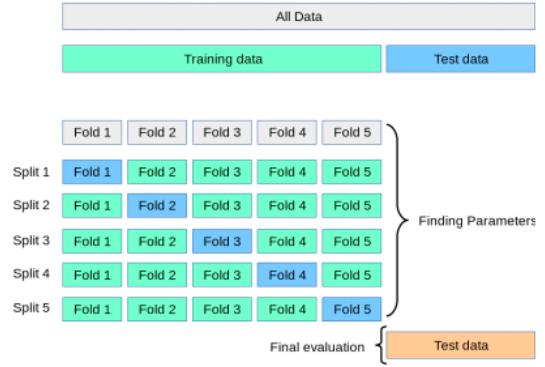
\includegraphics[width=0.8\textwidth]{images/Cross_Validation.png}
 \caption[k-fold Cross Validation.]{k-fold Cross Validation\protect\footnotemark}
 \label{fig:cross_val}
\end{figure}

\footnotetext{Librería Scikit-learn. \textit{Cross-Validation: evaluating estimator performance}. \url{https://scikit-learn.org/stable/modules/cross_validation.html}. (Consultado el 30 marzo de 2022).}

En conclusión, luego de realizar dichas iteraciones mediante k-fold Cross Validation, obtendremos la métrica de evaluación final para cada uno de las combinaciones de nuestros hiper-parámetros, y elegiremos los hiper-parámetros más óptimos (el que mejor métrica de evaluación nos haya dado). 

Una vez hallados los mismos, el último paso, como comentamos con el primer esquema, es realizar una evaluación final sobre el set de pruebas con los hiper-parámetros que encontramos, y de esta manera nos dará el accuracy (o la métrica de evaluación que elegimos) para los datos que el modelo no vió.

Un ejemplo de la utilización de estos esquemas para la evaluación de modelos, lo podemos observar en  \textit{\nameref{IMP_Modelo_clasificacion_KNN}}.\\

\paragraph{Los Problemas de ML: Overfitting y Underfitting.}\label{Over_y_under}

En esta sección vamos a nombrar y explicar algunos de los problemas clave en tareas de ML: overfitting y underfitting. Podemos observar un ejemplo de estos conceptos en la Figura \ref{fig:fitting}.

\begin{figure}[H]    %[H] es para que se ubique justo debajo del texto anterior.
 \centering
 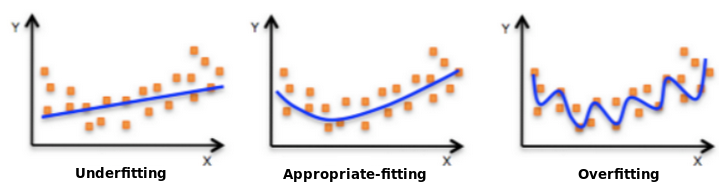
\includegraphics[width=0.9\textwidth]{images/Fitting.png}
 \caption{Overfitting y Underfitting\cite{apunte_uba}}
 \label{fig:fitting}
\end{figure}

\textbf{Overfitting}, o sobre-ajuste, es un problema clave en las tareas de aprendizaje automático supervisado.
Es el fenómeno que se detecta cuando un algoritmo de aprendizaje se ajusta/entrena tan bien al set de datos de entrenamiento que se memorizan el ruido y peculiaridades específicas de los datos de entrenamiento. Entonces, se vuelve difícil para el modelo generalizar a nuevos ejemplos que no estaban en el conjunto de entrenamiento. Es por esto que la precisión del modelo cae cuando se prueba en un conjunto de datos desconocido. De esta manera, termina siendo mayor la precisión en el entrenamiento que la precisión sobre los set de pruebas.

La cantidad de datos utilizados para el proceso de aprendizaje es fundamental en este contexto. Los conjuntos de datos pequeños son más propensos al overfitting que los conjuntos de datos grandes. El ajuste excesivo de los datos de entrenamiento conduce al deterioro de las propiedades de generalización del modelo y da como resultado un rendimiento o precisión del mismo poco fiable\cite{over_and_under}.

El concepto de overfitting está asociado a la complejidad del modelo. Un modelo excesivamente complejo puede ajustar tan bien como queramos al set de entrenamiento pero funcionar muy mal para el set de test\cite{apunte_uba}.

En cambio \textbf{Underfitting}, o sub-ajuste, es el opuesto de Overfitting. Esto ocurre cuando el modelo es incapaz de capturar la variabilidad de los datos. Se produce cuando el modelo es demasiado simple. Si nuestros puntos están distribuidos en forma curva, un modelo lineal es demasiado simple, no tiene el poder expresivo necesario para representar correctamente el set de entrenamiento\cite{apunte_uba}.

Por lo tanto, podemos decir que el modelo óptimo es aquel que tiene la complejidad necesaria para capturar lo que los datos expresan pero no más.

\cleardoublepage
\subsection{K-Nearest Neighbor (KNN).}

K-Nearest Neighbor o K Vecinos más cercanos (KNN), es un algoritmo ML que se puede usar tanto en tareas de regresión como de clasificación. En nuestra implementación, lo usaremos para resolver un problema de clasificación (ver \textit{\nameref{clasificacion}}). Como mencionamos anteriormente, en los problemas de clasificación la variable que se intenta predecir es discreta. En este tipo de problemas contamos con un set de entrenamiento en el cual para cada dato conocemos la clase a la cual pertenece el mismo, y queremos construir un modelo que nos permita clasificar automáticamente datos nuevos cuya clase desconocemos.

Como lo dice su nombre, el algoritmo KNN se basa en encontrar para un determinado punto m, sus K-vecinos más cercanos. Esto es asumiendo que nuestro set de datos está formado por un conjunto de m puntos en n dimensiones siendo todos los valores numéricos.\\

Para poder utilizar KNN hay que definir previamente dos hiper-parámetros:
\begin{itemize}
\item La métrica a usar para calcular las distancias.
\item El valor de k, es decir cuantos vecinos vamos a considerar.
\end{itemize}

Algo a destacar, es que KNN es un tipo de aprendizaje basado en la memoria, también llamado aprendizaje basado en instancias, que pertenece al aprendizaje perezoso (“lazy learning”). Esto quiere decir que KNN \textbf{no tiene una fase de entrenamiento}. ¿Qué quiere decir que KNN no tenga un proceso de entrenamiento?, y entonces en \textit{\nameref{IMP_Modelo_clasificacion_KNN}} ¿qué se hace realmente al utilizar la función \textit{.fit()} provista por sklearn?. A continuación se contestarán estas preguntas:

\begin{itemize}
\item \textbf{A nivel conceptual}, entrenar un clasificador significa tomar un conjunto de datos como entrada, y obtener a la salida un modelo clasificador identificado con distintos parámetros, los cuales son obtenidos en esta etapa de entrenamiento mediante iteraciones realizando cálculos numéricos o resolviendo problemas de optimización (como por ejemplo la obtención del mejor hiperplano en SVM o el ajuste de los pesos en redes neuronales artificiales). En el caso de KNN, el clasificador no se obtiene luego de iterar y obtener dichos parámetros, sino que se identifica por los propios datos de entrenamiento. Entonces, conceptualmente, entrenar un clasificador KNN simplemente requiere almacenar el conjunto de entrenamiento.

\item \textbf{A nivel de implementación}, evaluar un clasificador KNN en un nuevo punto de datos requiere buscar sus vecinos más cercanos en el conjunto de entrenamiento, lo que puede ser una operación costosa cuando nuestro conjunto de entrenamiento es grande. Existen varios métodos para acelerar esta búsqueda, que generalmente funcionan creando estructuras de datos basadas en el conjunto de entrenamiento. La idea general, es que parte del trabajo computacional necesario para clasificar nuevos puntos es común en todos los puntos. Por lo tanto, este trabajo se puede hacer con anticipación y luego reutilizarse, en lugar de repetirse para cada nueva instancia. De esta manera, en la fase de entrenamiento, al llamar a la función \textit{.fit()} de sklearn, lo que se hace internamente es guardar todo el set de entrenamiento completo mediante estructuras de datos que nos permitan minimizar los futuros cálculos de medición de distancias. Estas estructuras de datos suelen ser árboles kd (\textit{KD tree}) o árboles de bolas (\textit{Ball tree}). De esta manera, posteriormente a utilizar \textit{.fit()} utilizaremos \textit{.predict()}, y en este paso el cálculo de medición de distancias para el nuevo punto a clasificar será mucho más rápido.\\
\end{itemize} 

\subsubsection{Principal limitación KNN.}

Una de las principales limitaciones de KNN\cite{KNN_limitacion} es la \textbf{complejidad computacional requerida al trabajar con datasets de gran tamaño}. 

Esto ocurre debido a que, como mencionamos previamente, cada vez que se va a realizar una predicción para un nuevo punto del set de test, es necesario calcular las distancias entre este punto y todos los demás puntos del set de entrenamiento completo. Dichos cálculos llevan un gran costo computacional si se trata de un dataset de grandes dimensiones. 

Además, KNN requiere almacenar todos los datos de entrenamiento para funcionar, por lo que también existe un gran costo computacional en términos de almacenamiento. Es por esto que se recomienda utilizar datasets de pocas dimensiones para que el clasificador KNN complete su ejecución rápidamente. \\

\subsubsection{Funcionamiento y ejemplo de KNN.}

Luego de haber entrenado / construido nuestro modelo KNN habiendo previamente determinado el valor de k y la métrica de distancia a utilizar, el funcionamiento del algoritmo KNN para la predicción o clasificación de nuevas muestras es el siguiente: 

\begin{itemize}
\item Paso 1: Dado un nuevo punto de entrada del set de pruebas, se calculan las distancias entre este nuevo punto y todos los puntos del set de entrenamiento.
\item Paso 2: Se ordenan las distancias y se determinan los K vecinos más cercanos basándose en los valores mínimos de dichas distancias.
\item Paso 3: Se analiza la clase de esos vecinos y se asigna una clase para ese punto de entrada basado en el voto de la mayoría.
\item Paso 4: Se retorna la clase predicha.
\end{itemize}

A modo de ejemplo, veamos un caso en el cual usamos KNN para clasificación usando la distancia euclidiana como métrica para calcular las distancias. 

Como podemos ver en la Figura \ref{fig:KNN_example}, el conjunto de datos está etiquetado: uno es un cuadrado azul y otro es un triángulo rojo. El círculo verde es el punto que necesitamos clasificar. 

\begin{figure}[H]    %[H] es para que se ubique justo debajo del texto anterior.
 \centering
 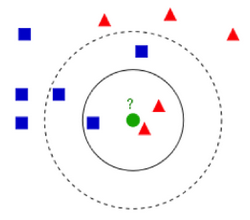
\includegraphics[width=0.4\textwidth]{images/KNN_Ejemplo.png}
 \captionsetup{justification=centering,margin=2cm}
 \caption{Ejemplo de Clasificación con KNN con K=3 (círculo con linea sólida) y K=5 (círculo con linea punteada), usando la distancia euclidiana como métrica de cálculo de distancias\cite{KNN_Ejemplo}.} 
 \label{fig:KNN_example}
\end{figure}

Viendo la Tabla \ref{table:2} observamos que:

\begin{itemize}
\item Si K = 1, tomamos únicamente el punto más cercano del círculo verde. Este punto es un triángulo rojo. Como es el único punto que vota, el punto verde a clasificar pertenece al triángulo rojo. De esta manera la probabilidad de que sea rojo es 1 y de que sea azul es 0.
\item Si K = 3, entonces hay 2 triángulos rojos y 1 cuadrado azul más cercano al punto verde Estos 3 puntos votan, por lo que el punto verde a clasificar pertenece al triángulo rojo. De esta manera la probabilidad de que sea rojo es 2/3  y de que sea azul es 1/3.
\item Si K = 5, entonces hay 2 triángulos rojos y 3 cuadrados azules más cercanos al punto verde. Estos 5 puntos votan, por lo que el punto verde a clasificar pertenece al cuadrado azul. De esta manera la probabilidad de que sea rojo es 2/5 y de que sea azul es 3/5 .
\end{itemize}

\begin{table}[h!]
\centering
\begin{tabular}{|p{2cm}|p{2cm}|p{2cm}|}
\hline
\textbf{K} & \textbf{P(Azul)} & \textbf{P(Rojo)} \\ [1ex] 
\hline
1 & 0 & 1 \\
\hline
3 & 1/3 & 2/3 \\
\hline
5 & 3/5 & 2/5 \\ [1ex] 
\hline
\end{tabular}
\caption{Probabilidad de pertenecer a cada clase para diferentes valores de k.}
\label{table:2}
\end{table}

Por lo tanto, podemos ver que KNN se basa esencialmente en un método estadístico. Cuando queremos simplemente clasificar un punto cuya clase no conocemos no hacen falta las probabilidades; podemos simplemente asignarlo a la clase con mayoría entre los k-vecinos del punto.\\

\subsubsection{Métrica de distancia a emplear.}

La función de distancia entre dos vectores $x$ e $y$ es una función $d(x,y)$ que define la distancia entre ambos vectores como un número real no negativo. Esta función es considerada como una métrica si satisface las siguientes 4 propiedades\cite{KNN_Ejemplo}: 

\begin{enumerate}
\item Valor no-negativo: La distancia entre $x$ e $y$ siempre es un valor mayor o igual a cero. 
$$d(x,y) \geq 0$$

\item Identidad de los indiscernibles: La distancia entre $x$ e $y$ es igual a cero si y sólo si $x$ es igual a $y$.
\[d(x,y) = 0, \text{   si  } x=y\]

\item Simetría:  La distancia entre $x$ e $y$ es igual a la distancia entre $y$ y $x$.
$$d(x,y) = d(y,x)$$

\item Desigualdad triangular: Considerando la presencia de un tercer punto $z$, la distancia entre $x$ e $y$ es siempre menor o igual que la suma de la distancia entre $x$ y $z$ y la distancia entre $y$ y $z$. 
$$d(x,y) \leq d(x,z) + d(y,z)$$
\end{enumerate}

De esta manera, puede usarse cualquier métrica para medir las distancias en KNN, siempre y cuando cumpla con las propiedades descritas anteriormente.

Dos de las distancias más utilizadas en la implementación de KNN son la distancia euclidiana y la distancia Manhattan. En  Figura \ref{fig:Man_euc} podemos observar gráficamente las diferencias entre las mismas.

\begin{figure}[H]    %[H] es para que se ubique justo debajo del texto anterior.
 \centering
 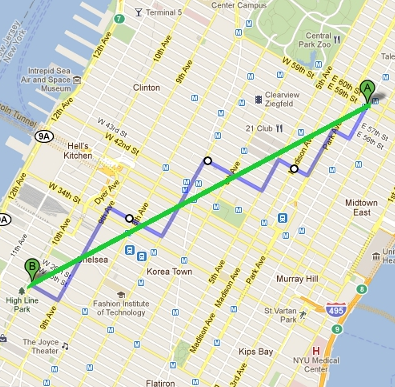
\includegraphics[width=0.6\textwidth]{images/Manhattan_Euclidiana.png}
 \captionsetup{justification=centering,margin=2cm}
 \caption{Distancia Manhattan vs Distancia Euclidiana\cite{apunte_uba}.} 
 \label{fig:Man_euc}
\end{figure}

La \textbf{distancia euclidiana}, o también conocida como Norma L2 o distancia de regla, es una extensión del Teorema de Pitágoras. Esta distancia representa la raíz de la suma al cuadrado de las diferencias absolutas entre los valores opuestos de los vectores. Considerando $x$ e $y$ como vectores a los cuales queremos calcular su distancia euclidiana, su cálculo se obtiene mediante la ecuación \ref{eq:ecuacion_1}.

\begin{equation}\label{eq:ecuacion_1}
d(x,y)=\sqrt{\sum_{i=1}^{n}|x_{i}-y_{i}|^2}   \qquad  \text{(Ver \cite{KNN_Ejemplo})}
\end{equation}

Donde $x=(x_{1},x_{2},..., x_{n})$, $y = (y_{1},y_{2},...,y_{n})$, y $n = \text{dimensiones de los puntos}$.

En la ecuación \ref{eq:ecuacion_2} y Figura \ref{fig:KNN_2_Dim} podemos observar el cálculo de la distancia euclidiana entre x e y  considerando un espacio bidimensional. Este es el cálculo que se realiza en la implementación de nuestro KNN, ya que utilizamos la distancia euclidiana como métrica, y únicamente contaremos con 2 ejes.

\begin{equation}\label{eq:ecuacion_2}
d(x,y)=\sqrt{(x_{1}-x_{2})^2 + (y_{1}-y_{2})^2}
\end{equation}

\begin{figure}[H]    %[H] es para que se ubique justo debajo del texto anterior.
 \centering
 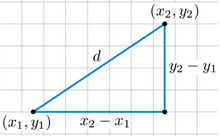
\includegraphics[width=0.4\textwidth]{images/KNN_2_Dim.png}
 \captionsetup{justification=centering,margin=2cm}
 \caption{Distancia Euclidiana en 2 dimensiones.} 
 \label{fig:KNN_2_Dim}
\end{figure}

En cambio, la \textbf{distancia Manhattan}\footnote{Su nombre es debido a que es la forma de calcular distancias en una ciudad con forma de grilla en la cual solo nos podemos mover por las calles en forma horizontal y vertical}, o también conocida como Norma L1 o distancia rectilínea, se calcula como la sumatoria de la diferencia absoluta entre los valores opuestos de los vectores.  Considerando $x$ e $y$ como vectores a los cuales queremos calcular su distancia Manhattan, su cálculo se obtiene mediante la ecuación \ref{eq:ecuacion_3}.

\begin{equation}\label{eq:ecuacion_3}
d(x,y)=\sum_{i=1}^{n}|x_{i}-y_{i}|  \qquad  \text{(Ver \cite{KNN_Ejemplo})}
\end{equation}

Donde $x=(x_{1},x_{2},..., x_{n})$, $y = (y_{1},y_{2},...,y_{n})$, y $n = \text{dimensiones de los puntos}$.

\cleardoublepage
\subsubsection{Eligiendo el valor de k: overfitting y underfitting.}

En el caso de KNN el único hiper-parámetro que manejamos -además de la métrica usada para la distancia-, es $k$. La elección del valor $k$ tendrá un impacto significativo en los resultados del algoritmo. 

Para determinar el valor óptimo para $k$ lo que se hace es probar diferentes valores de $k$ y ver cual es el que nos da mejores resultados. Aquí hay que tener un cierto cuidado ya que hay que entender qué implica aumentar o disminuir la cantidad de vecinos más cercanos.
Veamos en la Figura \ref{fig:KNN_k_1} qué pasa cuando usamos $k = 1$, es decir cuando a cada punto lo clasificamos únicamente en base al punto más cercano.

\begin{figure}[H]    %[H] es para que se ubique justo debajo del texto anterior.
 \centering
 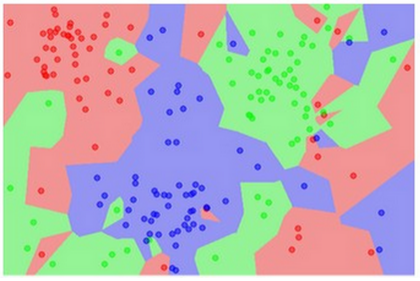
\includegraphics[width=0.7\textwidth]{images/KNN_k_1.png}
 \captionsetup{justification=centering,margin=2cm}
 \caption{KNN con k = 1. \cite{apunte_uba}} 
 \label{fig:KNN_k_1}
\end{figure}

En este caso nuestro el set de entrenamiento en KNN es simplemente perfecto porque dado un registro cualquiera, el más parecido es el registro mismo y, por lo tanto, vamos a tener 100\% de precisión para el set de entrenamiento. Sin embargo, esto no quiere decir que el algoritmo generalice bien y para el set de pruebas los resultados pueden ser catastróficos.

Lo que podemos ver es que la distribución que aprende nuestro clasificador no es homogénea, es decir que hay puntos de distintas clases mezclados en zonas en las cuales predomina otra clase, esto implica que nuestro clasificador va a funcionar muy bien para el set de entrenamiento pero no aprendió a generalizar y esto quiere decir que no va a ser muy bueno para predecir la clase de puntos nuevos que no hayamos observado en el set de entrenamiento. Esta es la definición de overfitting que discutimos en la sección previa (Ver \textit{\nameref{Over_y_under}}): cuando un algoritmo funciona bien para el set de entrenamiento y mal para datos nuevos. El concepto es que aprender a predecir el set de entrenamiento no es lo mismo que aprender a generalizar.

\cleardoublepage
Ahora veamos en la Figura \ref{fig:KNN_k_5} qué sucede con $k = 5$.

\begin{figure}[H]    %[H] es para que se ubique justo debajo del texto anterior.
 \centering
 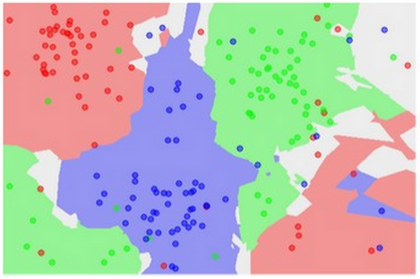
\includegraphics[width=0.7\textwidth]{images/KNN_k_5.png}
 \captionsetup{justification=centering,margin=2cm}
 \caption{KNN con k = 5. \cite{apunte_uba}} 
 \label{fig:KNN_k_5}
\end{figure}

Como podemos ver en la Figura \ref{fig:KNN_k_5} el clasificador aprendió a generar áreas más suaves y por consiguiente es un clasificador que generalizará mejor para predecir puntos que no estaban en el set de entrenamiento. Podriamos pensar entonces que es conveniente usar valores de k grandes como $k = 1000$ o incluso $k = n$ (donde $n$ es la cantidad de puntos de datos del set de entrenamiento). Sin embargo, al aumentar el valor de $k$ estamos dando cada vez mayor peso a las clases que tienen mayor cantidad de puntos en el set de entrenamiento, en el extremo si $k = n$ vamos a predecir para todos los puntos la clase que mayor cantidad de puntos tiene en el set de entrenamiento lo cual no es bueno. 

En resumen:
\begin{itemize}
\item Cuando $k$ es muy bajo, el algoritmo toma muy pocos puntos para clasificar un punto nuevo. Es un caso de overfitting. El modelo clasifica los puntos nuevos en base a muy poca evidencia. Nuestro algoritmo alucina, las fronteras se vuelven muy complejas, demasiado complejas para el set de datos que tenemos. 
\item Cuando $k$ es un número muy grande, KNN considera demasiados puntos para clasificar un punto nuevo. Este es un caso de underfitting, donde nuestro algoritmo tiene visión borrosa por estar mirando demasiados puntos, las fronteras entre nuestras clases se vuelven difusas y el poder expresivo del algoritmo es pobre. 
\end{itemize}

En definitiva, el $k$ óptimo en KNN es aquel que nos de un buen desempeño en cuanto a la precisión de clasificación para el mayor k posible. Una de las mejores formas para seleccionar nuestro $k$ óptimo, es utilizando el método de \textbf{Cross Validation} (ó validación cruzada): ver \textit{\nameref{Cross Validation}}.

\cleardoublepage
\subsection{K-means.}
K-means o K-medias, o también conocido como algoritmo de Lloyd, es un algoritmo de ML de clustering (ver \textit{\nameref{agrupacion}}). Como mencionamos anteriormente, en problemas de clustering contamos con datos que queremos dividir en grupos de forma automática. Estos datos no tienen etiquetas, no sabemos a qué grupo pertenecen. K-means nos permite encontrar cómo repartir m puntos en n dimensiones dentro de k clusters.

El nombre de K-means viene porque representa cada uno de los clusters por la media de sus puntos, es decir, por su centroide. Cada clúster, por tanto, es caracterizado por su centroide que se encuentra en el centro de los elementos que componen el clúster.

Para este algoritmo, el único hiper-parámetro que se necesita definir previamente es k, el número de clusters. Este k se puede obtener de distintas formas, en nuestra implementación utilizaremos el \textit{método del codo} para calcularlo. Antes de explicar en qué consiste este método, detallaremos el funcionamiento de k-means, su objetivo, sus desventajas y las mejoras que se pueden aplicar.

\subsubsection{Funcionamiento y ejemplo de K-means.}\label{K_means_funcionamiento}

Resumidamente, habiendo definido previamente nuestro k, el número de clusters, y teniendo como entrada nuestros puntos de datos $x_{1},...,x_{m}$, el funcionamiento de K-means consta de los siguientes 4 pasos \cite{K_means_review}:

\begin{itemize}
\item Paso 1: Se inicializan aleatoriamente los centroides $C_{1},...,C_{k}$ colocándose en posiciones al azar. Cada centroide $C_{j}$ pertenece a un cluster $j$ específico. 
\item Paso 2: Se asignan los puntos de datos a su cluster más cercano: Para esto, lo que se hace es, para cada punto de datos $x_{i}$, se calculan las distancias euclidianas con cada uno de los centroides $C_{j}$. Luego, se asigna cada punto de datos $x_{i}$ al cluster $j$, cuyo centroide $C_{j}$ es el más cercano al punto $x_{i}$ basándose en la mínima distancia euclidiana. Matemáticamente. se utiliza la Fórmula \ref{eq:ecuacion_1} para calcular la distancia euclidiana entre cada uno de nuestros puntos de datos $x_{i}$, y cada uno de nuestros centroides $C_{j}$, y obtener el mínimo valor. Reformulando dicha ecuación, nos quedaría la Fórmula \ref{eq:ecuacion_4}.   

\begin{equation}\label{eq:ecuacion_4}
d(x,C_{j})=\sqrt{\sum_{i=1}^{d}|x_{i}-C_{ji}|^2}  \qquad  \text{(Ver \cite{K_means_experiment})}
\end{equation}

Donde $d = \text{dimensiones de nuestros puntos de datos}$, $x_{i} = (x_{1},x_{2},...,x_{d})$ la posición de un punto $x$ de nuestro set de datos para la dimensión $i$, y $C_{ji} = (C_{11},C_{12},...,C_{kd})$ la posición de nuestro centroide $C$ del cluster $j$ para la dimensión $i$.
            
En la Fórmula \ref{eq:ecuacion_4}, podemos visualizar que los centroides tienen igual cantidad de dimensiones que nuestros puntos y, además, pueden o no coincidir con puntos de los datos. Un centroide que es también un punto de los datos se lo llama “clusteroid”. En general, no se pide que los centroides sean también puntos sino que se permite que tomen cualquier posición dentro del espacio de los datos.

\item Paso 3: Se actualizan las posiciones de los $C_{j}$ (centroides $C$ pertenecientes a los clusters $j$). De esta manera, se recalculan los centroides como el promedio de todos sus puntos (los que pertenecen a su cluster) de forma tal de minimizar la distancia desde el centroide a los puntos asignados al mismo. Como resultado, los centroides se mueven al centro promedio de los puntos a los que se les asignaron. Matemáticamente. se utiliza la Fórmula \ref{eq:ecuacion_5} para calcular, para cada cluster $j=(1,...,k)$ la nueva posición del centroide $C_{j}$, el cual se calcula como el promedio de todos los puntos $x_{i}$ asignados al cluster $j$ en el paso anterior.  

\begin{equation}\label{eq:ecuacion_5}
C_{j}(a)=\frac{1}{m_{j}}\sum_{x_{i} \in C_{j}}^{x_{m}}x_{i}(a),     \text{   para  } a = (1,...,d)
\end{equation}

Donde $d = \text{dimensiones de nuestros puntos de datos y centroides}$, $m_{j}$ = cantidad de puntos de nuestro set de datos pertenecientes al cluster $j$, $x_{i}(a)$ = posición de nuestro punto del set de datos $x_{i}$ para la dimensión $a$, y $C_{j}(a)= (C_{1}(1),C_{1}(2),...., C_{K}(D))$ la posición de nuestro centroide $C$ del cluster $j$ para la dimensión $a$.

\item Paso 4: Se repiten los pasos 2 y 3 hasta que los centroides convergen. La convergencia puede verificarse mediante la diferencia entre los centroides entre el paso anterior y el actual. Cuando los centroides prácticamente ya no cambian de posición o cuando los puntos de datos no cambian de cluster se declara la \textbf{convergencia} del algoritmo.\\

\end{itemize}

A modo de ejemplo, veamos un caso en el cual usamos K-means para clusterizar nuestros datos hasta llegar a su convergencia. 

En el ejemplo de la Figura \ref{fig:K_means_working_1}, nuestros datos tienen 2 dimensiones. Definiendo previamente nuestro k=2 (2 clusters), en el item \textbf{(1)} observamos dicha distribución de datos. Además, en este item se realiza la inicialización aleatoria de nuestros 2 centroides (triángulos rojo y amarillo). Todo esto involucra al \textbf{paso 1} del algoritmo k-means.  

\begin{figure}[H]    %[H] es para que se ubique justo debajo del texto anterior.
 \centering
 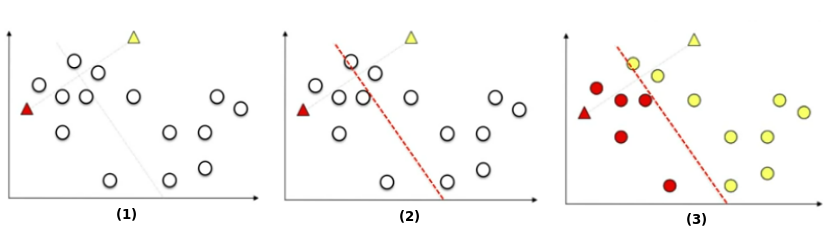
\includegraphics[width=1\textwidth]{images/K_Means_1.png}
 \captionsetup{justification=centering,margin=2cm}
 \caption{Algoritmo K-means.} 
 \label{fig:K_means_working_1}
\end{figure}

En el \textbf{paso 2}, lo que se tiene que hacer es, para cada uno de nuestros puntos de datos, averiguar a cuál centroide se asignará, basándonos en la distancia más cercana al mismo.
Al considerar la distancia euclidiana para este objetivo, en \textbf{(2)} dibujamos una línea roja imaginaria que divide en iguales distancias nuestros 2 centroides: partiendo de esta línea la distancia a ambos centroides es la misma. De esta manera, cada punto ubicado a la derecha de la linea pertenecerá al cluster amarillo (por tener menor distancia al centroide triángulo amarillo), y cada punto ubicado a la izquierda de la linea pertenecerá al cluster rojo (por tener menor distancia al centroide triángulo rojo). Esta asignación la observamos en el item \textbf{(3)}, que representa nuestra asignación inicial de nuestros puntos en los clusters. 

La línea roja es simplemente una referencia utilizada para una mejor comprensión gráfica, pero internamente esta asignación de puntos se realiza en base al cálculo de las distancias euclidianas mediante la Fórmula \ref{eq:ecuacion_4}. descrita anteriormente para el paso 2 de k-means.

Posteriormente pasamos al \textbf{paso 3} de k-means: la actualización de las posiciones de los centroides de los clusters. Lo que hacemos en \textbf{(4)} es mover los centroides al centro promedio de los puntos a los que se les asignaron. Para esto se utiliza la Fórmula \ref{eq:ecuacion_5} descrita anteriormente. Podemos observar las nuevas posiciones de los centroides en \textbf{(5)}. 
De esta forma, finalizamos la primera iteración de nuestro algoritmo. 

\begin{figure}[H]    %[H] es para que se ubique justo debajo del texto anterior.
 \centering
 \includegraphics[width=0.7\textwidth]{images/K_Means_2.png}
 \captionsetup{justification=centering,margin=2cm}
 \caption{Algoritmo K-means.}
\end{figure}

En la próxima iteración, tenemos la misma disposición de los puntos, solo que ahora tenemos dos nuevas posiciones para nuestros centroides. Ignoramos las clases que se asignaron para los puntos de nuestros datos ya que esta era una asignación del paso anterior: ahora nuestros centroides cambiaron y la asignación de clases también lo hará. Nuevamente trazamos la linea imaginaria \textbf{(6)} y realizamos la nueva asignación: los únicos puntos que cambiaron con respecto al paso anterior son los 2 amarillos ubicados en la parte superior, los cuales pasan a ser rojos \textbf{(7)}. Debido a que cambiaron de clase, entonces nuevamente vamos a actualizar las posiciones de nuestros centroides \textbf{(8)}, quedándonos distribuidos finalmente como \textbf{(9)}. De esta manera finalizamos la segunda iteración. 

\begin{figure}[H]    %[H] es para que se ubique justo debajo del texto anterior.
 \centering
 \includegraphics[width=0.7\textwidth]{images/K_Means_3.png}
 \captionsetup{justification=centering,margin=2cm}
 \caption{Algoritmo K-means.}
\end{figure}

\begin{figure}[H]    %[H] es para que se ubique justo debajo del texto anterior.
 \centering
 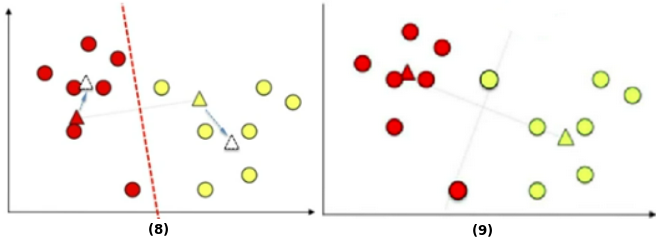
\includegraphics[width=0.7\textwidth]{images/K_Means_4.png}
 \captionsetup{justification=centering,margin=2cm}
 \caption{Algoritmo K-means.}
\end{figure}

Para la tercera iteración se vuelven a repetir los pasos 2 y 3: trazamos la línea de división de nuestros datos \textbf{(10)}, realizamos la nueva asignación de puntos \textbf{(11)} y observamos que cambiaron 2 puntos de clases.  Debido a que cambiaron de clase, entonces re-ubicamos los centroides nuevamente \textbf{(12)}, quedándonos finalmente como \textbf{(13)}.  De esta manera finalizamos la tercera iteración. 

\begin{figure}[H]    %[H] es para que se ubique justo debajo del texto anterior.
 \centering
 \includegraphics[width=0.7\textwidth]{images/K_Means_5.png}
 \captionsetup{justification=centering,margin=2cm}
 \caption{Algoritmo K-means.}
\end{figure}

\begin{figure}[H]    %[H] es para que se ubique justo debajo del texto anterior.
 \centering
 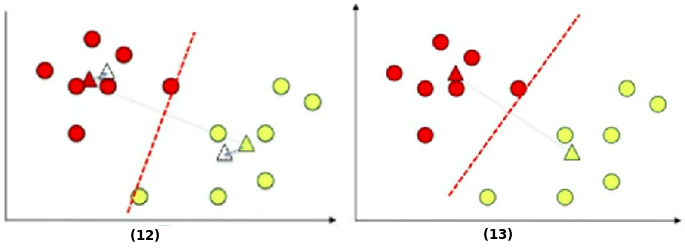
\includegraphics[width=0.7\textwidth]{images/K_Means_6.png}
 \captionsetup{justification=centering,margin=2cm}
 \caption{Algoritmo K-means.}
\end{figure}

Finalmente, en el ítem \textbf{(13)}, si ahora intentamos asignar nuevamente nuestros puntos de datos, observamos que ninguno cambiaría de color/clase. Los puntos rojos ya están del lado izquierdo de la linea, y los puntos amarillos ya están del lado derecho de la linea. Esto significa que si seguimos iterando nada cambiará, por lo que llegamos a la \textbf{convergencia} de nuestro algoritmo.

\cleardoublepage
\subsubsection{Objetivo de k-means y su función de coste.}

El objetivo de K-means es encontrar cómo repartir m puntos en n dimensiones dentro de k clusters de la “mejor forma posible”. 

¿A qué llamamos “de la mejor forma posible”?: se puede definir a cada cluster a partir de su centro (centroide), en cuyo caso la mejor distribución posible es aquella que minimiza la distancia entre cada punto del cluster y el centroide que se le asignó. Esto es lo que se conoce como \textbf{Inercia} (Inertia) o \textbf{WCSS} (within-cluster sum-of-squares, suma de cuadrados intra cluster), y es lo que busca \textit{minimizar} K-means.

A este criterio de Inercia también se lo considera como la \textbf{función de coste J}\footnote{La función de coste o también llamada función de distorsión u objetivo, es una función que trata de determinar la diferencia o el error entre el valor estimado / predicho por un modelo de machine learning y el valor real, con el fin de optimizar los parámetros en dicha función y obtener un error mínimo. En el caso de k-means, nuestros valores estimados son las posiciones de los centroides -los cuales tenemos que descubrir y encontrar los más óptimos / los que minimicen nuestra J- y nuestros valores reales son nuestros puntos del cluster.} de K-means, la cual se intenta \textit{minimizar}. 

Dicho de otra manera, el objetivo de k-means es encontrar la ubicación de los centroides que minimicen la inercia, esta será la posición óptima de los mismos.

La Inercia\cite{K_means_experiment} se puede reconocer como una medida de la coherencia interna de los clústeres, permitiendo medir qué tan bien K-means realiza la agrupación del conjunto de datos. La misma se calcula como la sumatoria de las diferencias de las distancias (generalmente euclidiana) al cuadrado entre cada uno de los puntos de datos $x_{i}$ pertenecientes a un cluster $j$ y el centroide al que fue asignado dicho punto, $C_{j}$: Fórmula \ref{eq:ecuacion_6}.

\begin{equation}\label{eq:ecuacion_6}
J = Inertia = WCSS = \sum_{C_{j}}^{C_{k}}  ( \sum_{xi \in C_{j}}^{x_{m}}||x_{i}-C_{j}||^2)
\end{equation}

Donde $k$ = número de centroides ó clusters, $m$ = cantidad de puntos de nuestro set de datos, $C_{j}$ = centroide de cluster $j$, y $x_{i}$ = punto $i$ de nuestro set de datos asignado a $C_{j}$. Además, el término $||x_{i}-C_{j}||$ se corresponde a la distancia euclidiana entre cada punto del set de datos, $x_{i}$, y el centroide que tiene asignado, $C_{j}$. Este cálculo se corresponde a la Fórmula \ref{eq:ecuacion_4} que obtuvimos anteriormente.

Considerando una inicialización aleatoria de nuestros centroides, y por ejemplo, definiendo que nuestro número de clusters es 3 ($k$ en kmeans = 3), entonces la Fórmula \ref{eq:ecuacion_6} se podría reescribir como la Fórmula \ref{eq:ecuacion_7}. Podemos observar que al variar la inicialización de nuestros centroides, las posiciones de nuestros $C_{j}$ cambiarían, por lo que nuestra $WSS$ sería distinta. 

\begin{equation}\label{eq:ecuacion_7}
WCSS =  \sum_{x_{i} \in C_{1}}||x_{i}-C_{1}||^2 + \sum_{x_{i} \in C_{2}}||x_{i}-C_{2}||^2 + \sum_{x_{i} \in C_{3}}||x_{i}-C_{3}||^2     \qquad  \text{(Ver \cite{K_means_elbow})}
\end{equation}

\cleardoublepage
Es importante entender la Fórmula \ref{eq:ecuacion_6} para comprender el problema genérico de clustering. Se sabe que hay k centroides y que cada uno de estos centroides puede estar en cualquier punto del espacio. El objetivo de k-means es \textbf{encontrar la posición óptima para estos centroides de forma tal de minimizar la distancia total entre los puntos y los centroides que se le han asignado}. Es evidente que cada punto debe estar asignado a su centroide más cercano para minimizar la distancia por lo que el problema puede resumirse a \textbf{encontrar la posición óptima para los k centroides}.

Obtener el mínimo valor de nuestro $WCSS$, o que es lo mismo que encontrar el mínimo global, es un proceso muy complejo debido a la inmensa cantidad de formas en las que nuestros m puntos de datos se pueden repartir en k clusters. En lugar de esto, k-means trata de encontrar una solución que, aun no siendo la mejor de entre todas las posibles, sea buena (óptimo local) y garantice un agrupamiento en el que los clusters sean poco dispersos y se encuentren separados entre sí.

Es de destacar que, suponiendo que tenemos $m$ puntos de datos y especificamos que este $m$ sea nuestro número de clusters ($k$ = $m$), entonces $WCSS$ será 0 ya que cada punto de nuestros datos actuará como centroide de sí mismo y la distancia euclidiana entre ellos será nula. De esta forma, cada cluster contendrá solo un punto. Esto idealmente es un cluster perfecto, pero no tiene ningún sentido tener tantos clusters como puntos de datos tengamos. Por lo tanto, existe un valor de umbral para $k$ que podemos encontrar utilizando el \textit{método del codo}, el cual veremos más adelante en \textit{\nameref{Elbow_Met}}).

\subsubsection{Posición inicial de los centroides.}\label{Posicion inicial centroides}

Al ser un algoritmo que encuentra un mínimo local, K-means es muy sensible a la posición inicial de los centroides. Una posible solución para no caer en un mínimo local malo es realizar varias ejecuciones de K-means con inicializaciones aleatorias para los centroides, idealmente ejecuciones en paralelo, y computar la función de coste $J$ para cada resultado final quedándonos con la mínima. 

La Figura \ref{fig:K_means_costo_1} muestra un ejemplo donde hay 4 clusters y varios puntos aislados en un plano bidimensional. La Figura \ref{fig:K_means_costo_2} muestra el resultado del mejor y peor costo. Se puede ver que el resultado del peor costo es realmente muy malo mientras que el resultado del mejor costo es lo que se esperaba obtener.  

\begin{figure}[H]    %[H] es para que se ubique justo debajo del texto anterior.
 \centering
 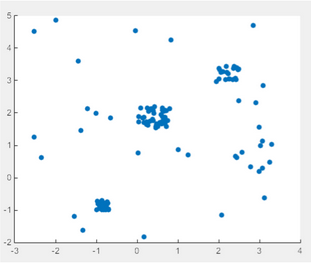
\includegraphics[width=0.4\textwidth]{images/K_means_costo_1.png}
 \captionsetup{justification=centering,margin=2cm}
 \caption{Ejemplo K-means. \cite{apunte_uba}}
 \label{fig:K_means_costo_1}
\end{figure}

\begin{figure}[H]    %[H] es para que se ubique justo debajo del texto anterior.
 \centering
 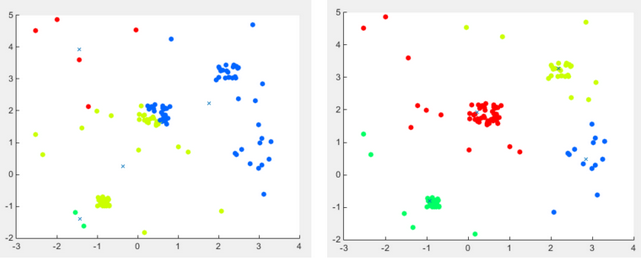
\includegraphics[width=0.9\textwidth]{images/K_means_costo_2.png}
 \captionsetup{justification=centering,margin=1cm}
 \caption{Ejemplo K-Means peor (izquierda) y mejor (derecha) costo. \cite{apunte_uba}}
 \label{fig:K_means_costo_2}
\end{figure}  

El gráfico de la Figura \ref{fig:K_means_costo_3} muestra el resultado de la función costo para 100 ejecuciones de K-Means, con un $k$ predefinido, y variando las inicializaciones de nuestros centroides. En el eje $x$ se representan las 100 ejecuciones de k-means, y en el eje $y$ encontramos la función de coste $J$ obtenida para cada ejecución. 

En la Figura \ref{fig:K_means_costo_4} podemos observar un histograma representando la cantidad de veces en porcentajes (eje $y$) que se observaron diferentes rangos de costo (eje $x$). Como se puede ver, afortunadamente los costos bajos son amplia mayoría, es decir que únicamente con algunas pocas inicializaciones desafortunadas K-means llega a un mínimo global muy malo. Esto quiere decir que una sola iteración de K-Means nos dará un buen resultado con una probabilidad alta y hacer un ciclo con unas pocas ejecuciones es más que suficiente para llegar a un excelente resultado.

\begin{figure}[H] %[H] es para que se ubique justo debajo del texto anterior.
\begin{minipage}[b]{0.5\linewidth}
\centering
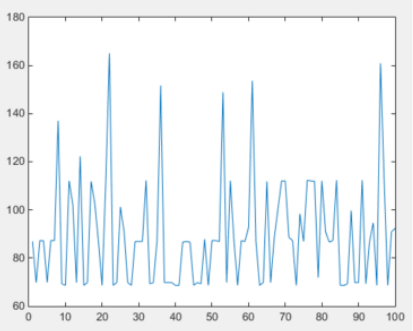
\includegraphics[width=\linewidth]{images/K_means_costo_3.png}
\caption{Costo en K-Means. \cite{apunte_uba}}
\label{fig:K_means_costo_3}
\end{minipage}
\hspace{0.5cm}
\begin{minipage}[b]{0.5\linewidth}
\centering
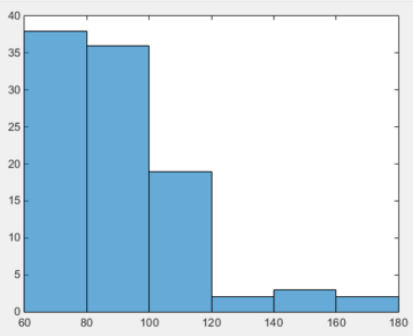
\includegraphics[width=\linewidth]{images/K_means_costo_4.png}
\caption{Histograma J en K-Means. \cite{apunte_uba}}
\label{fig:K_means_costo_4}
\end{minipage}
\end{figure}

\cleardoublepage
\subsubsection{Limitaciones K-means.}

K-means tiene tres principales limitaciones, las cuales describiremos a continuación.

\begin{enumerate}

\item \textbf{Outliers}: Un outlier es una observación atípica dentro de una muestra de datos que es notablemente diferente del resto. Los outliers representan errores en la medición, mala recolección de datos, o simplemente muestran variables no consideradas al recolectar los datos.
En k-means los outliers pueden incrementar la función de coste o Inercia. 

Varios investigadores observaron que, cuando los datos contienen outliers, existe una variación en el resultado que significa que no hay un resultado estable al realizar diferentes ejecuciones de k-means con los mismos datos\cite{K_means_review}. Por esta razón, es muy importante eliminar los outliers de nuestro conjunto de datos. Los valores atípicos se pueden eliminar aplicando técnicas de preprocesamiento en el conjunto de datos original.

\item \textbf{Número de los $k$ clusters}: Uno de los principales inconvenientes de K-means es la necesidad de determinar el número óptimo de los $k$ clusters por adelantado. Esto perjudica la eficacia del algoritmo ya que en la práctica, no se conoce a priori el número de clusters final. Este defecto lo perjudica al compararlo con otros algoritmos, ya que en muchos la inicialización del número de clusters no es necesaria. Todavía es un problema saber cuál es el número correcto de $k$ clusters que debemos asignar\cite{K_means_review}.

\item \textbf{Inicialización de los centroides}: Como vimos en la sección \textit{\nameref{Posicion inicial centroides}}, la selección inicial de los centroides dirige el proceso de K-means y las particiones resultantes y su efectividad están condicionadas a la elección de estos centroides\cite{K_means_experiment}. 
Existen numerosos estudios\cite{K_means_initial_centroids} que muestran que la performance de K-means es fuertemente dependiente de la estrategia de inicialización de la ubicación de los centroides a utilizar.

\end{enumerate}

Todas estas limitaciones descritas anteriormente fueron abordadas y resueltas en la implementación de k-means realizada para este proyecto de la siguiente forma:

\begin{itemize}

\item Para el primer problema, los outliers, se aplicó un pre-procesamiento de nuestros datos que permitió removerlos: ver \textit{\nameref{IMP_Modelo_clasificacion_KNN}}.

\item Para el problema de la determinación óptima y por adelantado del número de los $k$ clusters, se aplicó el \textit{método del codo}: ver \textit{\nameref{Elbow_Met}}.

\item Para el último caso de inicialización de los centroides, como mencionamos anteriormente, una de las soluciones para no caer en un mínimo local malo es realizar varias ejecuciones de K-means con inicializaciones aleatorias para los centroides, computar la función de distorsión J para cada resultado final y quedarnos con el mínimo. 

En la implementación de esta Tesis, se utilizó una estrategia más novedosa, inicializar nuestros centroides utilizando K-means++: ver \textit{\nameref{k_means_plus_plus}}. La ventaja de utilizar esta estrategia es que generalmente funciona mejor y más rápido que la detallada anteriormente, por lo que actualmente es uno de los métodos estándar para inicializar nuestros centroides en k-means. \cite{K_means_plus_plus}
\end{itemize}

\cleardoublepage
\paragraph{Obtención del k mediante Elbow Method.}\label{Elbow_Met}

Como se mencionó anteriormente, es necesario encontrar el valor óptimo de $k$. Un buen modelo k-means es uno que tenga la menor Inertia y un bajo número de clusters $k$. Sin embargo esto no es posible, ya que si $k$ aumenta, Inertia decrece.

\textit{Elbow method} o \textit{método del codo} nos permite determinar el óptimo valor de $k$, o dicho de otra forma, el óptimo número de clusters en los cuales nuestros puntos de datos serán clusterizados. Mediante este método lo que se hace es graficar cómo varía la función de costo o Inercia en función de $k$: recordemos que la Inercia se calcula mediante la Fórmula \ref{eq:ecuacion_6}. 

Luego de obtener este gráfico, se encuentra el punto ``del codo'', el cual indicará nuestro $k$ óptimo. Este es el punto después del cual la Inercia comienza a disminuir de forma lineal, o dicho de otra forma, el punto ``del codo'' indica que después de este punto, el cambio en la disminución del valor de la Inercia no es significativo. 

Veamos el siguiente ejemplo donde obtendremos nuestro $k$ óptimo en base al \textit{método del codo}: para los puntos de datos observados en la Figura \ref{fig:Elbow_1}, podemos observar visualmente 3 clusters separados, por lo que el número óptimo de clusters debería ser 3. En este caso es bastante sencillo observar esto, pero hay muchos casos donde no es fácil visualizar a simple vista el número de $k$ óptimo, y es por esto que el \textit{método del codo} es de gran utilidad. 

Utilizando esta técnica, graficamos la Inertia en función de $k$: iteramos valores de $k$ desde 1 hasta 9 y calculamos los valores de inercia para cada valor de $k$ dentro de ese rango, obteniendo el gráfico de la Figura \ref{fig:Elbow_2}.

\begin{figure}[H] %[H] es para que se ubique justo debajo del texto anterior.
\begin{minipage}[b]{0.5\linewidth}
\centering
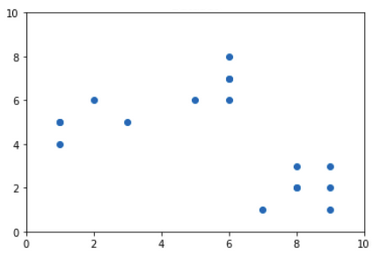
\includegraphics[width=\linewidth]{images/Elbow_1.png}
\caption{Puntos de datos.}
\label{fig:Elbow_1}
\end{minipage}
\hspace{0.5cm}
\begin{minipage}[b]{0.5\linewidth}
\centering
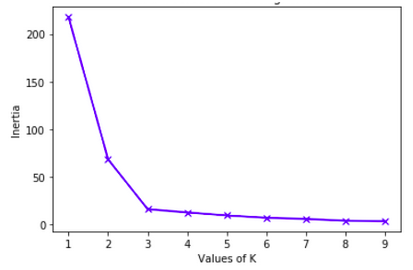
\includegraphics[width=\linewidth]{images/Elbow_2.png}
\caption{Método del codo usando Inercia.}
\label{fig:Elbow_2}
\end{minipage}
\end{figure}
 
De esta manera, concluimos que, para estos datos, viendo el gráfico de la Figura \ref{fig:Elbow_2}, el punto ``del codo'' está en $k=3$, siendo 3 nuestro $k$ óptimo. 

\cleardoublepage
En la Figura \ref{fig:Elbow_3} podemos visualizar los puntos de datos clusterizados para diferentes valores de $k$, observando de esta manera que con $k=3$ obtenemos la clusterización más óptima y lógica.

\begin{figure}[H]    %[H] es para que se ubique justo debajo del texto anterior.
 \centering
 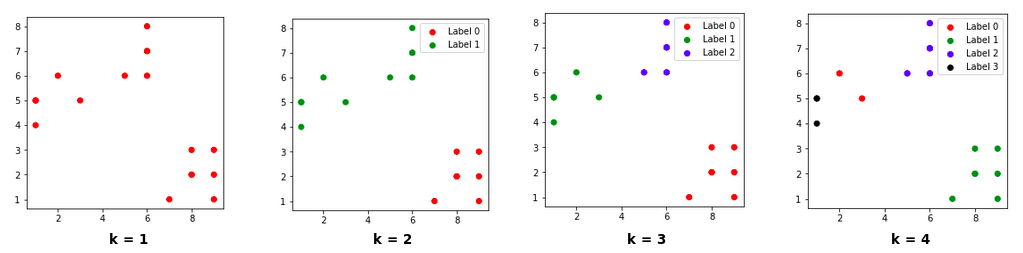
\includegraphics[width=1\textwidth]{images/Elbow_3.png}
 \captionsetup{justification=centering,margin=1cm}
 \caption{Puntos de datos clusterizados para diferentes valores de $k$.}
 \label{fig:Elbow_3}
\end{figure} 

\paragraph{Inicialización de los centroides: k-means++.}\label{k_means_plus_plus}

K-Means++\cite{K_means_plus_plus} es una variante de K-Means en donde lo único que cambia con respecto a este es la forma en que se inicializan los centroides (el paso 1 de k-means descrito en la sección \textit{\nameref{K_means_funcionamiento}}). Actualmente es uno de los métodos estándar para inicializar los centroides en k-means.

De esta manera, habiendo predefinido nuestro $k$, los pasos para inicializar nuestros centroides con k-means++ son:

\begin{enumerate}
\item Se elige un punto al azar como primer centroide. Este paso es el mismo que ocurre en k-means, solo que en este caso únicamente el primer centroide será elegido al azar.
\item Calculamos la distancia $D(x)$ entre cada punto de nuestros datos $x$ y su centroide. 
\item Uno de nuestros puntos de datos $x$ será elegido como el nuevo centroide. Este nuevo centroide será el que tenga la mayor distancia al cuadrado $D(x)^2$ con respecto a su centroide, es decir, el punto $x$ que tenga la distancia más lejana con su centroide. 
\item Repetimos los pasos 2 y 3 hasta que nuestros $k$ centroides sean asignados.
\end{enumerate}

La idea de K-means++ es asignar los centroides de forma espaciada, de esta forma el óptimo local obtenido por K-Means tiene una mayor probabilidad de estar cerca del óptimo global.

\cleardoublepage
En la secuencia de la Figura \ref{fig:K_means_plus_plus} podemos observar un ejemplo de asignación de centroides por medio de k-means ++, habiendo previamente definido $k=3$. Observamos que, a partir de la muestra de datos \textbf{(1)}, obtendremos la inicialización de nuestros centroides \textbf{(6)}.\\

\begin{figure}[H]    %[H] es para que se ubique justo debajo del texto anterior.
 \centering
 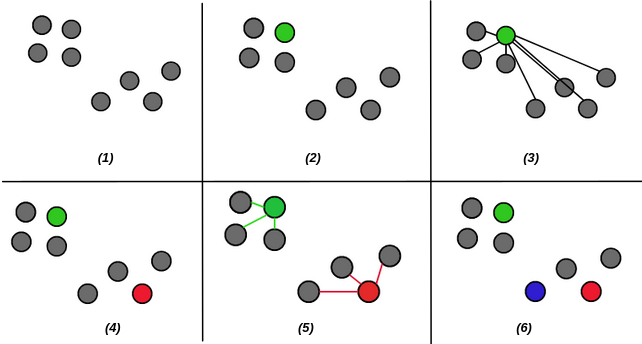
\includegraphics[width=0.8\textwidth]{images/K_means_plus_plus.png}
 \captionsetup{justification=centering,margin=1cm}
 \caption{Inicialización de centroides mediante K-means.}
 \label{fig:K_means_plus_plus}
\end{figure} 

En \textbf{(2)} se elige aleatoriamente un punto al azar como centroide inicial (en este caso el punto verde).
En \textbf{(3)} se calcula la distancia $D(x)$ entre cada uno de los puntos $x$ y su centroide. Para este caso únicamente tenemos el centroide verde. 
En \textbf{(4)} se encuentra al segundo centroide (rojo) de manera que esté alejado del centroide verde. Este segundo centroide es el punto x que tiene la mayor distancia al cuadrado $D(x)^2$ a su centroide.
En \textbf{(5)} se calculan nuevamente las distancias $D(x)$ entre cada uno de los puntos y su centroide más cercano.
Por último, en \textbf{(6)} finalizamos la inicialización de nuestros centroides encontrando al último y tercer centroide (azul). El mismo fue elegido ya que su punto $x$ es el que tiene la mayor distancia al cuadrado $D(x)^2$ a su centroide con respecto a cualquier otro punto y su centroide.

De esta manera, concluimos que K-means++ genera una inicialización más dispersa de los centroides iniciales comparándolo con el método de K-means estándar de inicialización aleatoria. El problema de K-Means++ es que para datos realmente masivos necesita hacer k iteraciones sobre los datos para elegir los centroides, tarea que es todavía más ineficiente cuando k es un número largo. Sin embargo, en general, K-Means++ genera una inicialización mejor para K-Means y esto permite no solo obtener una mejor solución final sino que también acelera la velocidad de convergencia del algoritmo.

\cleardoublepage
\subsection{Redes Neuronales.}
Este modelo es el utilizado para ....




\cleardoublepage
\section{Natural Language Processing.}\label{4.NaturalLanguageProcessing}

\colorbox{red}{FALTA}

\cleardoublepage

\subsection{Introducción.}
\colorbox{red}{FALTA}

\cleardoublepage

\subsection{Preprocesamiento de textos.}
\colorbox{red}{FALTA}

\cleardoublepage

\subsection{Similitud entre textos.}
\colorbox{red}{FALTA}

\cleardoublepage

\subsection{Técnicas para medir Similitud entre textos.}\label{Tecnicas_Simil_textos}
\colorbox{red}{FALTA}

\subsubsection{Cosine Similarity.}
\colorbox{red}{FALTA}

Cosine Similarity se basa en la medición del coseno del ángulo entre dos vectores proyectados en un espacio multidimensional para lograr medir la similitud de los documentos (un menor ángulo indica una mayor similitud). En este contexto, estos dos vectores representan matrices que contienen el recuento de palabras de dos documentos. Una de sus limitaciones es que  no tiene la habilidad de reconocer si las palabras que compara son semánticamente similares.

\cleardoublepage

\subsubsection{Word Mover's Distance (WMD).}
\colorbox{red}{FALTA}

Anteriormente, mencionamos que una de las limitaciones de Cosine Similarity es que no tiene habilidad de reconocer si las palabras que compara son semánticamente similares. En cambio, Word Mover's Distance (WMD) es un algoritmo más complejo que sí permite reconocer las relaciones semánticas; su limitación son las relaciones sintácticas (VER.........). WMD se basa en word embeddings y permite medir la distancia entre documentos (una menor distancia indica una mayor similitud).

\cleardoublepage

\subsection{Algoritmos de vectorización.}
\colorbox{red}{FALTA}

Previamente a utilizar Cosine Similarity y WMD para (-----completar-----) se debe emplear algún algoritmo de vectorización que permita representar las palabras de nuestros textos a un espacio vectorial. De esta forma Cosine Similarity y WMD podrán interpretarlos de la mejor manera. 
Como algoritmos de vectorización se utilizarán TF-IDF y Word Embeddings.

\subsubsection{TF-IDF.}
\colorbox{red}{FALTA}

El algoritmo TF-IDF asigna valores numéricos a las palabras en función de la frecuencia con que aparecen en los textos para medir la frecuencia de ocurrencia de un término en la colección de documentos, expresando  cuán relevante es una palabra para un documento en una colección. 

\cleardoublepage

\subsubsection{Word Embeddings.}
\colorbox{red}{FALTA}

Los Word Embeddings son necesarios para utilizar WMD.
Los Word Embeddings son una de las variantes más populares para representar textos.  Son vectores previamente entrenados y generados mediante un modelo de red neuronal secuencial; de esta manera son capaces de capturar los contextos de una palabra en el documento llegando a poder contener información semántica y sintáctica. 

\cleardoublepage

\paragraph{¿Cómo entrenar Word Embeddings?}
\colorbox{red}{FALTA}

\cleardoublepage

\section{Implementación.}\label{5.Implementacion}

La implementación de este Sistema se trabajó en dos grandes partes:
\begin{enumerate}
\item Obtención del modelo de clasificación. 

En esta primera parte se obtuvieron y preprocesaron datasets de Curriculum Vitae de distintos candidatos y descripciones de puestos de trabajo de IT publicados por distintas empresas, para luego ser comparados y obtener similitudes entre los textos utilizando las técnicas para medir distancias y obtener dichas similitudes (WMD y Cosine Similarity) y los algoritmos de vectorización (TF-IDF y Word Embeddings).

Una vez obtenidas estas mediciones de similitud entre los Curriculum Vitae de los candidatos y las descripciones de los puestos laborales de IT, estos valores se utilizaron para alimentar un algoritmo de clustering K-means que a su vez, con sus datos de salida (4 clusters), alimentan a un modelo de clasificación KNN. Finalmente, con este modelo KNN logramos, en base a los valores de similitud de nuevos candidatos, clasificar qué tan similares son dichos candidatos con respecto a la descripción de un puesto de IT: similitud escasa, similitud media, similitud alta, similitud muy alta.

Estos análisis se realizaron en documentos de Jupyter Notebook utilizando Python; y sirvieron para evaluar el comportamiento del modelo de clasificación y los distintos algoritmos de medición de similitudes para luego ser utilizados en la siguiente etapa. \\

\item Integración al Sistema Web. 

Etapa posterior a la primera parte. Una vez observado que los resultados fueron los esperables, lo que se hizo fue reutilizar las funciones que contenian la lógica de los distintos algoritmos utilizados junto con el modelo de clasificación KNN obtenidos previamente en la parte 1, para integrar todo esto en el sistema Web. Este sistema web está realizado en Django \footnote{Framework de desarrollo web de código abierto, escrito en Python, que respeta el patrón de diseño conocido como modelo–vista–controlador.}, y cuenta con una base de datos relacional que contiene la información de los candidatos y reclutadores junto con los Curiculum Vitae y puestos que hayan cargado. 

De esta manera, nuestro sistema cuenta con una interfaz gráfica permitiendo interactuar entre candidatos y reclutadores y, principalmente, permitiendo que el reclutador sea capaz de obtener un listado con los N candidatos más similes a un puesto determinado, y ordenados de mayor a menor de acuerdo a esta \textit{similitud}. Dicha \textit{similitud} representa el resultado obtenido de la clasificación por nuestro modelo KNN.

\end{enumerate}

\cleardoublepage

\subsection{Obtención del modelo de clasificación.}\label{5.1.Obtenciondelmodelopredictivo}

\subsubsection{Introducción.}
Como inicio definamos qué es un modelo. En nuestro caso, un modelo representa ....
Este modelo se construyó en base a ...
La implementación de este Sistema se realizó en Python...

\subsubsection{Esquema.}
Como podemos ver la figura \ref{fig:FlowCoreSystem} representa el procedimiento utilizado para la obtención de nuestro modelo de clasificación. 

\begin{figure}[H]    %[H] es para que se ubique justo debajo del texto anterior. 
  \centering
  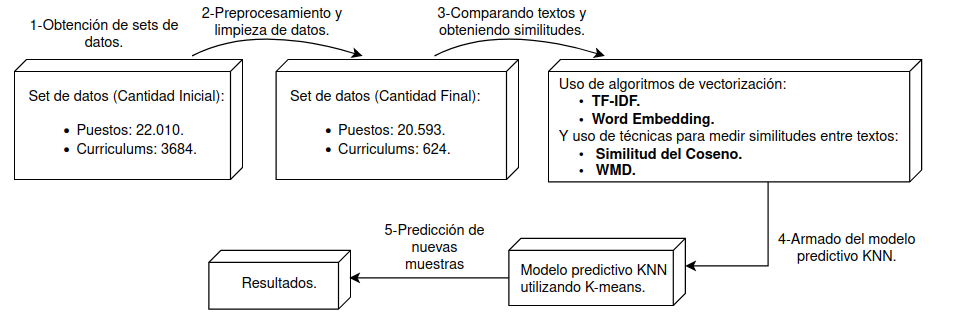
\includegraphics[width=1\textwidth]{images/flow-core.png} 	%Incluyendo imagen Flow Core.
  \caption{Pipeline Flow para la obtención del modelo de clasificación KNN}  
  \label{fig:FlowCoreSystem}
\end{figure}

\cleardoublepage

\subsubsection{Obtención de sets de datos.}
En primer lugar debemos definir qué es un set o conjunto de datos.
Un set o conjunto de datos es una tabla de una base de datos o, matemáticamente, una matriz estadística de datos. Cada columna de la tabla representa una variable del set de datos; y cada fila representa a un miembro determinado del mismo.

Para este Proyecto utilizamos dos grandes sets de datos que se obtuvieron mediante la recolección de distintos archivos alojados en la Web, los cuales estan descriptos a continuación.

\paragraph{Curriculum Vitae.}
Los set de datos de Curriculum Vitae de los candidatos se obtuvieron de las siguientes fuentes:

\begin{enumerate}
\item 228 Curriculums en formato docx y posteriormente convertidos a pdf, obtenidos del sitio Kaggle\footnote{\url{https://www.kaggle.com/palaksood97/resume-dataset}}. Estos pdfs son candidatos de la India con experiencia en el rubro de IT.
\item 2484 Curriculums en formato CSV, obtenidos del sitio Kagle\footnote{\url{https://www.kaggle.com/snehaanbhawal/resume-dataset}}. Este CSV cuenta con curriculums vitae obtenidos del sitio web de postulación de trabajos 'livecareer.com'.
\item 962 Curriculumns en formato CSV, obtenidos del sitio Kaggle\footnote{\url{https://www.kaggle.com/gauravduttakiit/resume-dataset}}. Este CSV cuenta con curriculums vitae repartidos en distintas categorías de IT.
\item 10 Curriculums en formato PDF, los cuales los cuales fueron obtenidos como ejemplos mediante una recolección propia de distintos sitios web. 
\end{enumerate}

\paragraph{Descripciones Puestos Laborales.}

Los set de datos de descripciones de puestos laborales se obtuvieron de las siguientes fuentes:

\begin{enumerate}
\item 22.000 descripciones en formato CSV; obtenido del sitio Kaggle\footnote{\url{https://www.kaggle.com/PromptCloudHQ/us-technology-jobs-on-dicecom}}. El CSV cuenta con descripciones de puestos obtenidos del sitio web de USA de postulación de trabajos del rubro de IT 'Dice.com'.
\item 10 descripciones en formato CSV; obtenidas como ejemplos mediante una recolección propia del sitio Indeed\footnote{\url{https://www.indeed.com/q-USA-jobs.html}} para puestos de trabajo de IT.
\end{enumerate}

\cleardoublepage

\subsubsection{Preprocesamiento y limpieza de datos.}
Previamente a utilizar las técnicas para medir distancias y obtener similitudes entre textos (WMD y Cosine Similarity) y los algoritmos de aprendizaje (KNN y K-Means) necesitamos que los datos que comparemos e introduzcamos en los algoritmos estén lo más limpios posible; ya que de lo contrario las mismos podrían clasificar o predecir de forma errónea. Este análisis previo sobre los datos debe ser minucioso ya que puede haber valores incoherentes o absurdos.

El procedimiento para la Limpieza de los Curriculum Vitae y las descripciones de los puestos laborales fue el siguiente:

\begin{enumerate}
\item Convertimos todo a minúscula.
\item Eliminamos datos no relevantes para nuestros análisis (mails y páginas web).
\item Eliminamos signos de puntuación y caracterés especiales (incluyendo números).
\item Eliminamos stop words.
\item Eliminamos common words no relevantes para nuestros análisis.
\item Aplicamos Lematización y Tokenización.
\item Eliminamos repetidos.
\item Obtenemos y usamos bi-gramas.
\end{enumerate}

Luego de aplicar preprocesamiento y limpieza de datos nos quedarán los siguientes tamaños de nuestros datasets:
\begin{itemize}
\item 624 curriculums vitae de candidatos (en formato pdf y csv).
\item 20593 descripciones de puestos de IT (en formato csv).
\end{itemize}

\cleardoublepage

\subsubsection{Cantidad final del set de datos y su uso en las distintas etapas.}

El total de 624 curriculums vitae de candidatos y 20593 descripciones de duestos de IT que mencionamos previamente, serán utilizados para el entrenamiento y obtención de vectores mediante TF-IDF (para el posterior cálculo de Cosine Similarity) y para el entrenamiento de Word2Vec y obtención de los Word Embeddings (para el posterior cálculo de WMD).

Por otro lado, para calcular Cosine Similarity y WMD, para utilizarlos en K-means y para entrenar a nuestro algoritmo KNN, utilizaremos únicamente una porción de nuestros datasets:

1-Para el cálculo de Cosine Similarity y WMD:
\begin{itemize}
\item 301 curriculums vitae de candidatos.
\item 201 descripciones de puestos de IT.
\end{itemize}
Nota: No obstante, al realizar los cálculos de distancias compararemos cada curriculum vitae con cada Job Description, obteniendo un dataframe total de 3131 filas con sus respectivo valores de WMD y Cosine Sim.

2-Para el uso de K-means y entrenamiento con KNN (eliminamos un curriculum vitae y una descripción de puesto IT que los utilizamos en '3-'):
\begin{itemize}
\item 300 curriculums vitae de candidatos.
\item 200 descripciones de puestos de IT.
\end{itemize}        
Nota: como se comentó previamente, nos quedarán 3000 filas / puntos para usar en K-means y entrenar KNN; llegando a representar estos 3000 puntos en un plano de 2 dimensiones.

3-Para la clasificación de nuevas muestras mediante KNN:
\begin{itemize}
\item 1 curriculum vitae de candidatos.
\item 1 descripción de puesto de IT.
\end{itemize}
Nota: como se comentó previamente, nos quedarán 131 filas para clasificar.

¿Por qué utilizamos solo una porción de nuestros datasets?: Esto es debido a los drawbacks de WMD y KNN.
\begin{itemize}
\item WMD: posee una alta complejidad en el cálculo de la distancia, teniendo un tiempo de ejecución muy elevado. Como ejemplo, al correrlo localmente, el cálculo de WMD para 3131 filas tardó 7 horas; frente a los 3 segundos que tardó el cálculo de Cosine Similarity para la misma cantidad de filas.
\item KNN: KNN es una gran opción para datasets pequeños con pocas variables de entrada; pero tiene problemas cuando la cantidad de entradas es muy grande. En grandes dimensiones, los puntos que pueden ser similares pueden tener distancias muy grandes. Además, cada vez que se va a hacer una predicción con KNN, busca al vecino más cercano en el conjunto de entrenamiento completo. Por esto, se debe utilizar un dataset pequeño para que el clasificador KNN complete su ejecución rápidamente.
\end{itemize}
En conclusión, al utilizar solo una porción de nuestros datasets para obtener los distintos cálculos de distancias y entrenar KNN, el cálculo de WMD se podrá realizar en un tiempo finito, y nuestro clasificador KNN funcionará rápida y eficientemente al realizar predicciones.

\cleardoublepage

\subsection{Comparando textos y obteniendo similitudes.}
\colorbox{red}{FALTA}

Previamente a utilizar Cosine Similarity y WMD para obtener las medidas de similitud entre los textos, se debe emplear algún algoritmo de vectorización que permita representar las palabras de nuestros textos a un espacio vectorial. De esta forma Cosine Similarity y WMD podrán interpretarlos de la mejor manera.  Como mencionamos previamente, como algoritmos de vectorización se utilizarán TF-IDF y Word Embeddings. 

\cleardoublepage

\subsection{Armado del modelo de clasificación KNN.}\label{IMP_Modelo_clasificacion_KNN}
\colorbox{red}{FALTA}

Una vez obtenidas estas mediciones de similitud entre los Curriculum Vitae de los candidatos y las descripciones de los puestos laborales de IT, estos valores se utilizarán para alimentar un algoritmo de clustering K-means que a su vez, con sus datos de salida (4 clusters), alimentarán a un modelo de clasificación KNN. Finalmente, con este modelo KNN lograremos, en base a los valores de similitud de nuevos candidatos, clasificar qué tan similares son dichos candidatos con respecto a la descripción de un puesto de IT: similitud escasa, similitud media, similitud alta, similitud muy alta.

\cleardoublepage

\subsection{Clasificación de nuevas muestras y resultados obtenidos.}\label{5.4.Predicciondenuevasmuestrasyresultadosobtenidos}

\colorbox{red}{FALTA}

\cleardoublepage

\subsection{Integración al Sistema Web.}\label{5.5.IntegracionalSistemaWeb}
\colorbox{red}{FALTA}

Anteriormente lo que se hizo fue un análisis mediate documentos en Jupyter Notebooks para evaluar el comportamiento del modelo de clasificación y los distintos algoritmos de medición de similitudes. 

Al observar que los resultados fueron los esperables, lo que se hizo en esta última etapa fue reutilizar las funciones que contenian la lógica de los distintos algoritmos utilizados junto con el modelo de clasificación KNN obtenidos en la fase previa, para integrar todo esto en el sistema Web. 

Como mencionamos previamente, este sistema web está realizado en Django, y cuenta con una base de datos relacional que contiene la información de los candidatos y reclutadores junto con los Curiculum Vitae y puestos que hayan cargado. 

De esta manera, nuestro sistema cuenta con una interfaz gráfica permitiendo interactuar entre candidatos y reclutadores y, principalmente, permitiendo que el reclutador sea capaz de obtener un listado los N candidatos más similes a un puesto determinado, y ordenados de mayor a menor de acuerdo a esta \textit{similitud}. Dicha \textit{similitud} representa el resultado obtenido de la clasificación por nuestro modelo KNN.

El sistema web contará con 2 tipos de usuario: 
\begin{itemize}
\item Candidato: quienes cargarán en el sistema sus Curriculum Vitae y aplicarán a los distintos puestos disponibles.
\item Reclutador: quienes cargarán en el sistema los puestos de trabajo que tengan disponibles y podrán consultar, entre otras cosas, un listado con los N candidatos más similes a un puesto determinado, y ordenados de mayor a menor de acuerdo a esta \textit{similitud}.
\end{itemize}

\cleardoublepage

\subsubsection{Base de datos.}

Nuestros datos los almacenaremos en una base de datos \colorbox{red}{FALTA definir cual}. 

Para modelar y gestionar nuestros datos utilizamos el modelo relacional \footnote{Una base de datos relacional es un conjunto de una o más tablas estructuradas en registros (líneas) y campos (columnas), que se vinculan entre sí por un campo en común.}.

\colorbox{red}{Sacar la mayoría del documento modelo-entidad-relacion-case-method-richar-barker.pdf} 

Para comprender los datos que se almacenan en dicha base de datos, los representaremos utilizando un diagrama entidad relación \footnote{Un modelo entidad-relación es una herramienta para el modelo de datos, la cual facilita la representación de entidades de una base de datos.}.
Previamente a esto explicaremos los elementos del diagrama de entidad relación: 

\colorbox{red}{FALTA PONER IMAGEN CON LOS ELEMENTOS: Entidad rectángulo, Unión entre entidades son} \\ \colorbox{red}{las lineas que puede ser obligatoria u opcional, cardinalidad son los 1:M / 1:1 / M:M}

\begin{itemize}
\item Entidad: objeto concreto o abstracto que figura en nuestra base de datos. Por ejemplo una entidad puede ser un alumno, un cliente, una empresa, etc. Dentro de las entidades estan los atributos, atributos principales o clave primaria (PK) y atributos foraneos o clave secundaria (FK).  Las entidades que necesitamos para crear nuestra BD son: Candidato, Puesto, Reclutador y Candidato\_Puesto -entidad intermedia entre Candidato y Puesto-.
\item Unión entre entidades: pueden ser obligatorias u opcionales. En nuestro diagrama nuestras uniones son todas opcionales, ya que el reclutador puede o no CARGAR un puesto, el candidato puede o no APLICAR a un puesto y a su vez el puesto puede o no ser aplicado por un candidato. 
\item Cardinalidad: Relación entre entidades o mapeo. La cardinalidad es el tipo de relación entre entidades. Observando la figura \ref{fig:Cardinalidad} y considerando que los rectángulos azules son una entidad y los naranjas son otra entidad observamos que pueden haber 4 tipos de cardinalidades posibles:

\begin{enumerate}
\item Uno a uno: a cada entidad azul le corresponde solo una entidad naranja.
\item Uno a muchos: a cada entidad azul le corresponde una o varias entidades naranjas.
\item Muchos a uno: a cada entidad naranja le corresponde una o varias entidades azules.
\item Muchos a muchos: las entidades azules pueden tener varias entidades naranjas y las entidades naranjas también pueden tener varias entidades azules.
\end{enumerate}
\end{itemize}

\begin{figure}[H]    %[H] es para que se ubique justo debajo del texto anterior. 
  \centering
  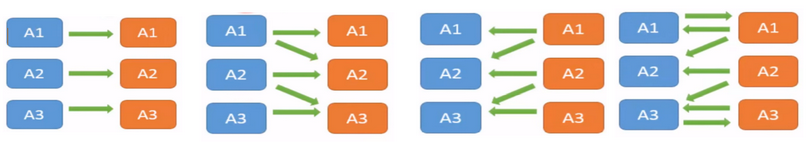
\includegraphics[width=1\textwidth]{images/Cardinalidad.png}
  \caption{Tipos de cardinalidad.}  
  \label{fig:Cardinalidad}
\end{figure}

La cardinalidad entre nuestras entidades son:
\begin{itemize}
\item Entre Candidato y Puesto existe una relación muchos a muchos (M:M), ya que un candidato puede aplicar a M puestos y un puesto puede ser aplicado por M candidatos. Es por esto que se creó la tabla intermedia Candidato\_Puesto conllevando dos relaciones uno a muchos (1:M) con Puesto y Candidato.
\item Entre Reclutador y Puesto existe una relación de uno a muchos (1:M), ya que un reclutador puede cargar M puestos, y un puesto pertenece a un solo reclutador.
\end{itemize}

En cuanto a las claves pueden haber dos tipos. Por un lado está la clave primaria o atributo principal (PK)  es única y toda entidad debe tener la suya. Pueden haber múltiples PKs; estas se llaman PKs compuestas. Y por el otro está la clave secundaria o atributo foráneo (FK). Estas claves identifican a una entidad externa en otra, utilizándose para generar relaciones entre nuestras entidades. Si tenemos una clave FK en una entidad, significa que dicha clave FK es clave PK en otra entidad.


El diagrama de relación que utilizamos para nuestro trabajo lo observamos en la figura \ref{fig:Entity_Relation}.

\begin{figure}[H]    %[H] es para que se ubique justo debajo del texto anterior. 
  \centering
  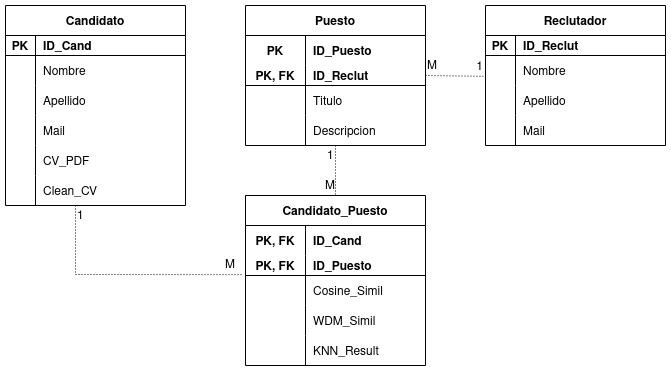
\includegraphics[width=1\textwidth]{images/BD_Entity_Relation.png}
  \caption{Diagrama de relación utilizado.}  
  \label{fig:Entity_Relation}
\end{figure}

\cleardoublepage

\subsubsection{Secciones del sistema}

Para registrarse o loguearse al sistema, se implementará la interfaz provista en la figura \ref{fig:Vista_Registro}.

\begin{figure}[H]    %[H] es para que se ubique justo debajo del texto anterior. 
  \centering
  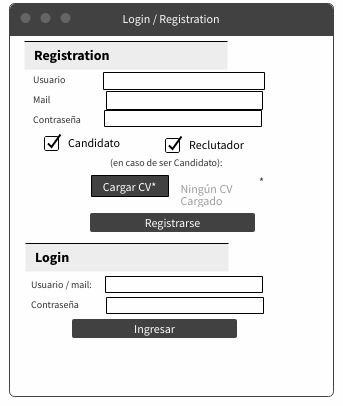
\includegraphics[width=1\textwidth]{images/Vista_Registro.png}
  \caption{Logueo y Registración.}  
  \label{fig:Vista_Registro}
\end{figure}

\colorbox{red}{ES UN BOCETO, FALTA PONER LA IMAGEN REAL}

El Candidato tendrá acceso al menú indicado en la figura \ref{fig:Vista_Candidato}. 

\begin{figure}[H]    %[H] es para que se ubique justo debajo del texto anterior. 
  \centering
  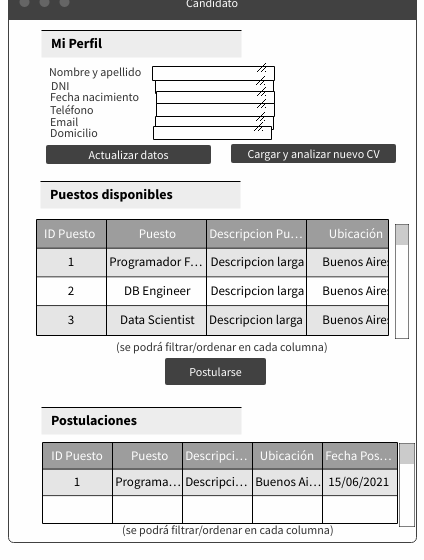
\includegraphics[width=1\textwidth]{images/Vista_Candidato.png}
  \caption{Vista del Candidato.}  
  \label{fig:Vista_Candidato}
\end{figure}

\colorbox{red}{ES UN BOCETO, FALTA PONER LA IMAGEN REAL}

Por su parte, el Reclutador tendrá acceso al menú indicado en la figura \ref{fig:Vista_Reclutador}. 

\begin{figure}[H]    %[H] es para que se ubique justo debajo del texto anterior. 
  \centering
  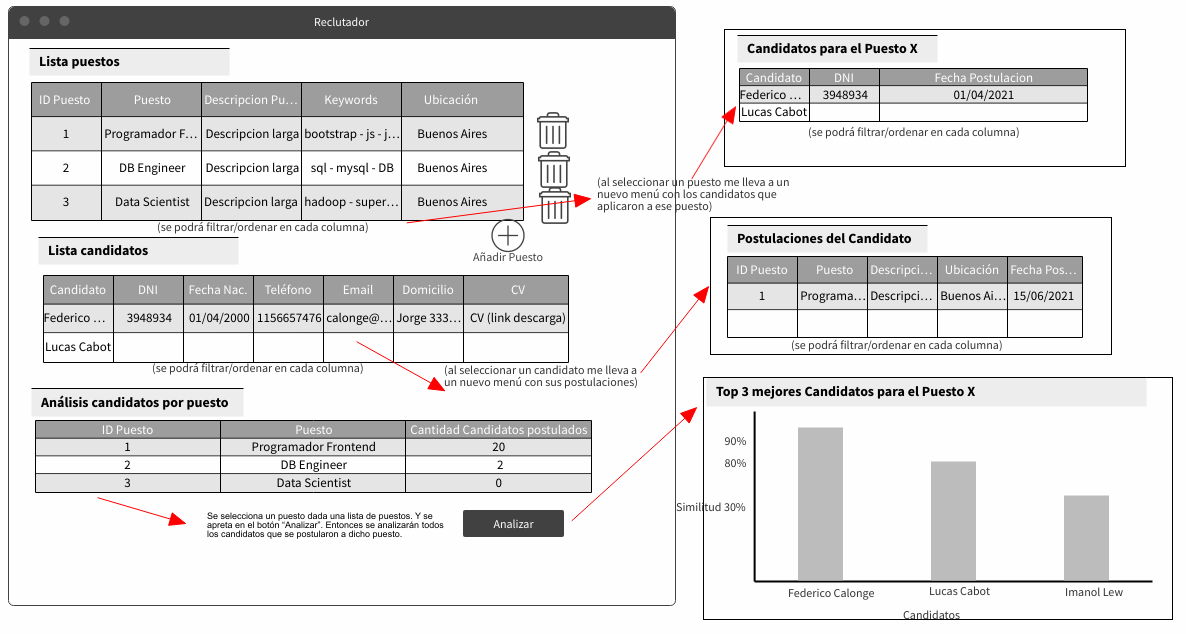
\includegraphics[width=1\textwidth]{images/Vista_Reclutador.png}
  \caption{Vista del Reclutador.}  
  \label{fig:Vista_Reclutador}
\end{figure}

\colorbox{red}{ES UN BOCETO, FALTA PONER LA IMAGEN REAL}

\cleardoublepage

\subsubsection{Manejo de los datos.}
\colorbox{red}{FALTA}

\cleardoublepage

\paragraph{Modelado.}
\colorbox{red}{FALTA}

\cleardoublepage

\paragraph{Filtrado.}
\colorbox{red}{FALTA}

\cleardoublepage

\paragraph{Visualización.}
\colorbox{red}{FALTA}

\cleardoublepage

\subsection{Pipeline Flow final del Sistema.}
\colorbox{red}{FALTA}

Una vez que el reclutador dentro de la sección observada en la figura \ref{fig:Vista_Reclutador} haga click en "Analizar", el sistema reflejará el pipeline indicado en la figura \ref{fig:Pipeline_Final} para obtener como resultado un listado con los N candidatos más similes a un puesto determinado, y ordenados de mayor a menor de acuerdo a esta \textit{similitud}. Dicha \textit{similitud} representa el resultado obtenido de la clasificación por nuestro modelo KNN.


\begin{figure}[H]    %[H] es para que se ubique justo debajo del texto anterior. 
  \centering
  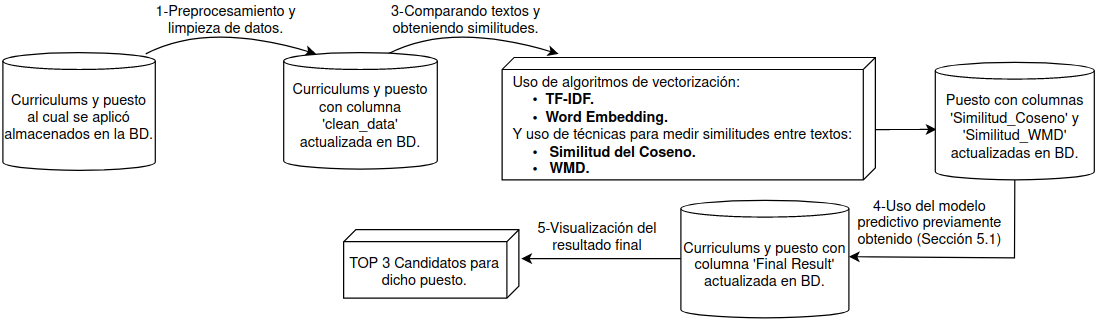
\includegraphics[width=1\textwidth]{images/Pipeline_Final.png}
  \caption{Pipeline Flow final del Sistema.}  
  \label{fig:Pipeline_Final}
\end{figure}

\cleardoublepage

\subsection{Conclusiones.}
\colorbox{red}{FALTA}

\cleardoublepage

\subsection{Caso de Uso.}
\colorbox{red}{FALTA}

\cleardoublepage

\subsection{Limitaciones del sistema.}

Las limitaciones del sistema son las siguientes:
\begin{itemize}
\item Solo acepta curriculums en formato PDF.
\item Curriculums y Puestos de trabajo en idioma inglés. 
\item Curriculums y Puestos de trabajo de IT. 
\end{itemize}

\cleardoublepage

\section{Próximos pasos.}  
\colorbox{red}{FALTA - acá poner mejoras}

\cleardoublepage

\section{Anexos.}
\colorbox{red}{FALTA}

\cleardoublepage


\begin{thebibliography}{9}

\bibitem{Similarity_calculation}
Pinky Sitikhu, Kritish Pahi, Pujan Thapa, \& Subarna Shakya. (2019, Octubre). \textit{A Comparison of Semantic Similarity Methods for Maximum Human Interpretability}. IEEE International Conference on Artificial Intelligence for Transforming Business and Society. (pp. 1-4).

\bibitem{jobs_future}
World Economic Forum. (2020, Octubre). \textit{The Future of Jobs Report}. (pp. 29-31).

\bibitem{wmd_paper}
Matt Kusner, Yu Sun, Nicholas Kolkin, \& Kilian Weinberger. (2015, Julio). \textit{From word embeddings to document distances}. International Conference on Machine Learning. (pp. 957–966).

\bibitem{similarity_survey}
Jiapeng Wang, \& Yihong Dong. (2020, Agosto). \textit{Measurement of Text Similarity: A Survey}. Information 2020. 11(9). (pp. 1-8, 13,14).

\bibitem{cosine_sim_1}
Baoli Li, \& Liping Han. (2013, Octubre). \textit{Distance Weighted Cosine Similarity Measure for Text Classification}. IDEAL2013 Conference. (pp. 1,2).

\bibitem{cosine_sim_2}
Chunjie Luo, Jianfeng Zhan, Lei Wang, \& Qiang Yang. (2017, Octubre). \textit{Cosine Normalization: Using Cosine Similarity Instead of Dot Product in Neural Networks}. (pp. 1,2).

\bibitem{cosine_sim_3}
Dani Gunawan, C A Sembiring, \& Mohammad Andri Budiman. (2018, Marzo). \textit{The Implementation of Cosine Similarity to Calculate Text Relevance between Two Documents}. 2nd International Conference on Computing and Applied Informatics 2017. Journal of Physics Conference Series. 978(1). (pp. 1-2).

\bibitem{seleccion_reclutamiento_1}
Derek S. Chapman, \& Jane Webster. (2003, Junio-Septiembre). \textit{The Use of Technologies in the Recruiting, Screening, and Selection Processes for Job Candidates}. International journal of selection and assessment. 11(2/3). (pp. 113-114, 117-119).

\bibitem{seleccion_reclutamiento_2}
Pshdar Abdalla Hamza, Baban Jabbar Othman, Bayar Gardi, Sarhang Sorguli, Hassan Mahmood Aziz, Shahla Ali Ahmed, Bawan Yassin Sabir, Nechirwan Burhan Ismael, Bayad Jamal Ali, \& Govand Anwar. (2021, Mayo-Junio).
\textit{Recruitment and Selection: The Relationship between Recruitment and Selection with Organizational Performance}. International journal of Engineering, Business and Management (IJEBM). 5(3). (pp. 1-6).

\bibitem{apunte_uba}
Luis Argerich, Natalia Golmar, Damián Martinelli, Martín Ramos Mejía, \& Juan Andrés Laura. (2019, Enero). \textit{75.06, 95.58 Organización de Datos}. Apunte del Curso Organización de Datos, Universidad de Buenos Aires, Facultad de Ingenieria. (pp. 4-8,351,352,377-379, 387-389,470-477). 

\bibitem{estudio_eye_tracking}
Ladders Company. (2018). \textit{Eye-Tracking Study}. (pp. 2,6).

\bibitem{trabajos_relacionados_1}
Riza Tanaz Fareed, Sharadadevi Kaganurmath, \& Rajath V. (2021, Agosto). \textit{Resume Classification and Ranking using KNN and Cosine Similarity}. International Journal of Engineering Research \& Technology (IJERT). 10(8). (pp. 192-194).

\bibitem{trabajos_relacionados_2}
Senthil Kumaran V, \& Annamalai Sankar. (2013, Mayo). \textit{Towards an automated system for intelligent screening of candidates for recruitment using ontology mapping (EXPERT)}. International Journal of Metadata, Semantics and Ontologies. 8(1). (pp. 56-64).

\bibitem{ontology_mapping}
Nuno Silva, \& Joao Rocha. (2003). \textit{Ontology Mapping for Interoperability in Semantic Web} , IADIS International Conference WWW/Internet (ICWI), Portugal. (pp. 1).

\bibitem{trabajos_relacionados_3}
Wahiba Ben Abdessalem Karaa, \& Nouha Mhimdi. (2011) \textit{Using ontology for resume annota-tion}. International Journal of Metadata, Semantics and Ontologies. 6(3). (pp. 166-174).

\bibitem{trabajos_relacionados_4}
Duygu Çelik, Askýn Karakas, Gülsen Bal, Cem Gültunca, Atilla Elçi, Basak Buluz, \& Murat Can Alevli. (2013, Septiembre). \textit{Towards an Information Extraction System Based on Ontology to Match Resumes and Jobs}. Computer Software and Applications Conference Workshops (COMPSACW), IEEE 37th. (pp. 333-338).

\bibitem{trabajos_relacionados_5}
Frank Färber, Tim Weitzel, \& Tobias Keim. (2003, Agosto). \textit{An automated recommendation approach to selection in personnel recruitment}. 9th Americas Conference on Information Systems (AMCIS). (pp. 1-11).

\bibitem{trabajos_relacionados_6}
Chirag Daryania, Gurneet Singh Chhabrab, Harsh Patel, Indrajeet Kaur Chhabrad, \& Ruchi Patel. (2020). \textit{An Automated Resume Screening System using Natural Language Processing and Similarity}. Topics In Intelligent Computing And Industry Design. 2(2). (pp. 99-103).

\bibitem{trabajos_relacionados_7}
Juneja Afzal Ayub Zubeda, Momin Adnan Ayyas Shaheen, Gunduka Rakesh Narsayya Godavari, \& Sayed ZainulAbideen Mohd Sadiq Naseem. (2016, Mayo). \textit{Resume Ranking using NLP and Machine Learning}. Proyecto de Tesis para carrera de grado \textit{Bachiller en Ingeniería}. School of Engineering and Technology Anjuman-I-Islam’s Kalsekar Technical Campus. (pp. 1-3).

\bibitem{trabajos_relacionados_8}
Jai Janyani, Kartik Agarwal, \& Abhishek Sharma. (2018). \textit{Automated Resume Screening System}. Proyecto de Tesis para carrera de grado \textit{Bachiller en Tecnología}. Rajasthan Technical University. (pp. 5, 9-15).

\bibitem{trabajos_relacionados_9}
V. V. Dixit, Trisha Patel, Nidhi Deshpande, \& Kamini Sonawane. (2019, Abril). \textit{Resume Sorting using Artificial Intelligence}. International Journal of Research in Engineering, Science and Management. 2(4). (pp. 423-425).

\bibitem{trabajos_relacionados_10}
Dr. K.Satheesh, A.Jahnavi, L Aishwarya, K.Ayesha, G Bhanu Shekhar, \& K.Hanisha. (2020). \textit{Resume Ranking based on Job Description using SpaCy NER model}. International Research Journal of Engineering and Technology (IRJET). 7(5). (pp. 74-77).

\bibitem{trabajos_relacionados_11}
Paolo Montuschi, Valentina Gatteschi, Fabrizio Lamberti,   Andrea Sanna, \&  Claudio Demartini. (2014, Septiembre-Octubre). \textit{Job recruitment and job seeking processes: how technology can help}. IT Professional. 16(5). (pp. 41-49).

\bibitem{trabajos_relacionados_12}
Leila Yahiaoui, Zizette Boufaïda, \& Yannick Prié. (2006). \textit{Semantic Annotation of Documents Applied to E-Recruitment}. SWAP 2006, the 3rd Italian Semantic Web Workshop. (pp. 1-6).

\bibitem{trabajos_relacionados_13}
Rémy Kessler, Nicolas Béchet, Mathieu Roche, Juan Manuel Torres-Moreno, \& Marc El-Bèze. (2012). \textit{A hybrid approach to managing job offers and candidates}. Information Processing \& Management. 48(6). (pp. 1124-1135).

\bibitem{trabajos_relacionados_14}
Pradeep Kumar Roy, Sarabjeet Singh Chowdhary, \& Rocky Bhatia. (2020). \textit{A Machine Learning approach for automation of Resume Recommendation system}. International Conference on Computational Intelligence and Data Science (ICCIDS). Procedia Computer Science. 167. (pp. 2318-2327).

\bibitem{trabajos_relacionados_15}
Ioannis Paparrizos, B. Barla Cambazoglu, \& Aristides Gionis. (2011). \textit{Machine learned job recommendation}. 5th ACM Conference on Recommender Systems, ACM. (pp. 325-328).

\bibitem{sistema_recomendacion}
Paul Resnick, \& Hal R. Varian. (1997). \textit{Recommender Systems}. Communications of the ACM40. (pp. 56-59).

\bibitem{intro_algos_ML}
M. Emre Celebi, Michael W. Berry, Azlinah Mohamed, \& Bee Wah Yap. (2020). Libro \textit{Supervised and Unsupervised Learning for Data Science}. (pp. 3,4,14,15).

\bibitem{aprendiz_transd}
Karthik Tangirala. (2011). \textit{Semi-supervised and transductive learning algorithms for predicting alternative splicing events in genes}. Proyecto de Tesis para carrera de grado \textit{Master of Science}. Kansas State University. (pp. 1-4).

\bibitem{cross_validation}
Daniel Berra. (2018). \textit{Cross-Validation}. Libro \textit{Reference Module in Life Sciences}. Data Science Laboratory, Tokyo Institute of Technology. (pp. 1-5).

\bibitem{preprocessing}
S. B. Kotsiantis, D. Kanellopoulos, \& P. E. Pintelas. (2006). \textit{Data Preprocessing for Supervised Leaning}. International Journal of Computer Science. 1(1). (pp. 111,112,116). 

\bibitem{metrics_clustering_1}
Stephen Bradshaw, \& Colm O’Riordan. (2018). \textit{Evaluating Better Document Representation in Clustering with Varying Complexity}. In Proceedings of the 10th International Joint Conference on Knowledge Discovery, Knowledge Engineering and Knowledge Management 2018. 1. (pp. 199-201).

\bibitem{metrics_clustering_2}
Julio-Omar Palacio-Niño, \& Fernando Berzal. (2019, Mayo). \textit{Evaluation Metrics for Unsupervised Learning Algorithms}. (pp. 1-6).

\bibitem{metrics_clasification}
Nathalie Japkowicz. (2006, Mayo). \textit{Why Question Machine Learning Evaluation Methods (An Illustrative Review of the Shortcomings of Current Methods)}. (pp. 1-5)

\bibitem{metrics_regression}
Alexei Botchkarev. (2018, Septiembre). \textit{Performance Metrics (Error Measures) in Machine Learning Regression, Forecasting and Prognostics: Properties and Typology}. Interdisciplinary Journal of Information, Knowledge, and Management, 2019. 14. (pp. 1-8).

\bibitem{over_and_under}
Haider Khalaf Jabbar, \& Rafiqul Zaman Khan. (2014). \textit{Methods to avoid over-fitting and under-fitting in supervised machine learning (comparative study)}. (pp. 163-165)

\bibitem{KNN_limitacion}
Zhou Yong,  Li Youwen, \& Xia Shixiong. (2009, Marzo). \textit{An Improved KNN Text Classification Algorithm Based on Clustering}. Journal of Computers. 4(3). (pp. 230, 233). 

\bibitem{KNN_Ejemplo}
Haneen Arafat Abu Alfeilat, Ahmad B.A. Hassanat, Omar Lasassmeh, Ahmad S. Tarawneh, Mahmoud Bashir Alhasanat, Hamzeh S. Eyal Salman, \& V.B. Surya Prasath. (2019, Diciembre). \textit{Effects of Distance Measure Choice on K-Nearest Neighbor Classifier Performance: A Review}. Libro \textit{Big Data}. 7(4). (pp. 1-9).

\bibitem{K_means_experiment}
Boyang Li. (2018, Febrero). \textit{An Experiment of K-Means Initialization Strategies on Handwritten Digits Dataset}. Intelligent Information Management. 10. (pp. 43-46). 

\bibitem{K_means_elbow}
Mengyao Cui. (2020). \textit{Introduction to the K-Means Clustering Algorithm Based on the Elbow Method}. Accounting, Auditing and Finance. 1. (pp. 5-8).

\bibitem{K_means_review}
Shraddha Shukla, \& Naganna S. (2014). \textit{A Review On K-means Data Clustering Approach}. International Journal of Information \& Computation Technology. 4(17). (pp. 1847-1849, 1852, 1853).

\bibitem{K_means_initial_centroids}
Kodinariya, T.M. (2014). \textit{Survey on Exiting Method for Selecting Initial Centroids in K-Means Clustering}. International Journal of Engineering Development and Research. 4(2). (pp. 2865-2868).

\bibitem{K_means_plus_plus}
David Arthur, \& Sergei Vassilvitskii. (2007, Enero). \textit{K-Means++: The Advantages of Careful Seeding}. SODA '07: Proceedings of the 18th annual ACM-SIAM symposium on Discrete algorithms. (pp. 1027-1035).

\end{thebibliography}

\end{document}
%Para poner en Las citas del anexo --> información\cite{iot}. 